\pdfoutput=1
\pdfinfoomitdate=1
\pdftrailerid{}
\pdfsuppressptexinfo=15
\documentclass[indonesian]{shinybook}
\usepackage{tikz}
\usepackage{pgfplots}
\usepgfplotslibrary{groupplots}
\pgfplotsset{compat=1.18}
\usetikzlibrary{intersections,calc}
\usetikzlibrary{arrows.meta, decorations.markings}
\usepackage{glossaries-extra}
\usepackage{needspace}

\newcommand{\half}{\frac{1}{2}}
\newcommand{\N}{\mathbb{N}}
\newcommand{\Z}{\mathbb{Z}}
\newcommand{\Q}{\mathbb{Q}}
\newcommand{\R}{\mathbb{R}}
\newcommand{\Rb}{\overline{\mathbb{R}}}
\newcommand{\bR}{\overline{\mathbb{R}}}
\newcommand{\F}{\mathbb{F}}
\newcommand{\1}{\mathbb{1}}
\newcommand{\linop}{\mathcal{L}}
\newcommand{\Rnn}{\mathbb{R}^{n\times n}}
\newcommand{\Cnn}{\mathbb{C}^{n\times n}}
\newcommand{\E}{\mathbb{E}}
\usepackage{pgffor}
\foreach \x in {A,...,Z}{%
    \expandafter\xdef\csname cal\x\endcsname{\noexpand\ensuremath{\noexpand\mathcal{\x}}}
}

\renewcommand{\implies}{\Rightarrow}
\newcommand{\setto}{\rightrightarrows}
\newcommand{\equivalent}{\Leftrightarrow}
\newcommand{\eps}{\varepsilon}
\renewcommand{\phi}{\varphi}
\newcommand{\supp}{\operatorname{\mathrm{supp}}}
\renewcommand{\div}{\operatorname{\mathrm{div}}}
\newcommand{\dom}{\operatorname{\mathrm{dom}}}
\renewcommand{\ker}{\operatorname{\mathrm{ker}}}
\newcommand{\conv}{\operatorname{\mathrm{conv}}}
\newcommand{\rg}{\operatorname{\mathrm{rg}}}
\newcommand{\graph}{\operatorname{\mathrm{graph}}}
\newcommand{\tr}{\operatorname{\mathrm{tr}}}
\newcommand{\epi}{\operatorname{\mathrm{epi}}}
% Never redefine TeX's primitive \span: amsmath alignment environments use it.
% Use \spann for the linear-span operator in reader prose and formulae.
\newcommand{\sign}{\operatorname{\mathrm{sign}}}
\DeclareMathOperator{\Id}{\mathrm{Id}}
\newcommand{\prox}{\mathrm{prox}}
\newcommand{\proj}{\mathrm{proj}}
\newcommand{\spann}{\operatorname{\mathrm{span}}}
\newcommand{\Lloc}{L^1_{\mathrm{loc}}}
\newcommand{\Cinf}{C^\infty_0}

% Nama lingkungan dilokalkan; penomoran dan topologi sumber dipertahankan.
\newtheorem{theorem}{Teorema}[chapter]
\newtheorem{lemma}[theorem]{Lema}
\newtheorem{cor}[theorem]{Korolari}
\theoremstyle{definition}
\newtheorem{defn}[theorem]{Definisi}
\newtheorem{prop}[theorem]{Proposisi}
\newtheorem{example}[theorem]{Contoh}
\newtheorem{assumption}[theorem]{Asumsi}
\newtheorem{exercise}[theorem]{Latihan}
\newtheorem*{rem}{Catatan}

\crefname{theorem}{teorema}{teorema}
\Crefname{theorem}{Teorema}{Teorema}
\crefname{lemma}{lema}{lema}
\Crefname{lemma}{Lema}{Lema}
\crefname{cor}{korolari}{korolari}
\Crefname{cor}{Korolari}{Korolari}
\crefname{prop}{proposisi}{proposisi}
\Crefname{prop}{Proposisi}{Proposisi}
\crefname{defn}{definisi}{definisi}
\Crefname{defn}{Definisi}{Definisi}
\crefname{example}{contoh}{contoh}
\Crefname{example}{Contoh}{Contoh}
\crefname{assumption}{asumsi}{asumsi}
\Crefname{assumption}{Asumsi}{Asumsi}
\crefname{rem}{catatan}{catatan}
\Crefname{rem}{Catatan}{Catatan}
\crefname{exercise}{latihan}{latihan}
\Crefname{exercise}{Latihan}{Latihan}

\renewcommand{\proofname}{Bukti}
\renewcommand{\contentsname}{Daftar Isi}
\renewcommand{\figurename}{Gambar}

\newcommand{\norm}[1]{\|#1\|}
\newcommand{\abs}[1]{\left|#1\right|}
\newcommand{\inner}[2]{\left\langle#1 , #2\right\rangle}
\newcommand{\dual}[1]{\langle #1 \rangle}
\newcommand{\setof}[2]{\left\{#1 \;\middle|\; #2\right\}}
\newcommand{\wkto}{\rightharpoonup}
\DeclareMathOperator{\Exp}{\mathbb{E}}
\DeclareMathOperator{\Var}{\mathbb{V}}
\DeclareMathOperator{\Cov}{\mathrm{Cov}}
\newcommand{\Prob}{\mathbb{P}}

\usepackage{enumerate}
\newcommand{\weaki}{\protect{\u{\i}}}
\AtBeginEnvironment{remark}{\small}

\ifdefined\OIntegratedReader
  % Keep examples as ordinary theorem blocks in the tagged master. The legacy
  % mdframed/tablefootnote patches interfere with the synchronized latex-lab
  % hooks, while no canonical body calls \tablefootnote.
\else
  \usepackage{mdframed}
  \mdfdefinestyle{examplebg}{
      backgroundcolor=structure!7,%
      hidealllines=true,%
      splittopskip=\topskip,
      frametitleaboveskip=0,
      frametitlebelowskip=0,
      innertopmargin=-.3em,%
      innerbottommargin=.7em,%
      innerleftmargin=.7em,%
      innerrightmargin=.7em,%
  }
  \surroundwithmdframed[style=examplebg]{example}
  \usepackage{tablefootnote}
  \makeatletter
  \AfterEndEnvironment{mdframed}{%
   \tfn@tablefootnoteprintout%
   \gdef\tfn@fnt{0}%
  }
  \makeatother
\fi

\usepackage{enumitem}
\setlist[enumerate]{label=(\roman*)}
\usepackage{scrhack}

\newcommand{\ie}{\textit{yaitu}}
\newcommand{\eg}{\textit{misalnya}}
\newcommand{\cf}{\textit{bandingkan}}
\newcommand{\emptyarg}{\,\cdot\,}
\newcommand{\dd}{\mathrm{d}}
\newcommand{\todo}[1]{{\color{red}Perlu dikerjakan: #1}}
\newcommand{\Oc}{\mathcal{O}}
\newcommand{\Lc}{\mathcal{L}}
\newcommand{\Gc}{\mathcal{G}}
\newcommand{\Ic}{\mathcal{I}}
\newcommand{\Pc}{\mathcal{P}}
\newcommand{\Mc}{\mathcal{M}}
\renewcommand{\epsilon}{\varepsilon}
\newcommand{\diag}{\mathrm{diag}}

\microtypesetup{expansion=false}
\emergencystretch=2em

\title{Optimisasi Konveks}
\subtitle{Prakata dan Bab 1--2: Prasyarat dan Kekonveksan\\Edisi Bahasa Indonesia}
\author{Andreas Habring}
\date{Sumber edisi v1: 13 Juli 2026}
\publishers{\small
Terjemahan lengkap bahasa Indonesia dari prakata dan Bab 1--2 \emph{Lecture Notes: Convex Optimization}, arXiv:2607.11664v1.\\
Karya sumber dan terjemahan/adaptasi ini tersedia berdasarkan CC BY 4.0; perubahan matematis dijelaskan secara terbuka.\\
Edisi mandiri ini bukan karya resmi atau dukungan Andreas Habring maupun TU Graz.}
\hypersetup{
    pdftitle={Optimisasi Konveks -- Prakata dan Bab 1--2: Prasyarat dan Kekonveksan -- Edisi Bahasa Indonesia},
    pdfauthor={Andreas Habring},
    pdflang={id-ID},
}

\begin{document}
\maketitle

\frontmatter
\chapter*{Tentang unit ini}
Unit ini menerjemahkan secara utuh prakata, Bab 1 ``Preliminaries'', dan Bab 2
``Convexity'' dari Andreas Habring, \emph{Lecture Notes: Convex Optimization},
arXiv:2607.11664v1. Batas ini mencakup halaman cetak 1--29 dan melengkapi
Bab 3--9 yang sudah diterjemahkan sebelumnya.

Tiga berkas sumber berwenang untuk unit ini dibekukan sebagai berikut:
\begin{center}
\begin{tabular}{@{}ll@{}}
\texttt{preface.tex} & \texttt{d6ec9d0522446fc65f3868d0b7cd1d22}\\
                     & \texttt{1462c3099fbd0b2d6ea412ab53315967}\\[0.25em]
\texttt{preliminaries.tex} & \texttt{8c1e4bdad36f2dcb57867c475afa5adc}\\
                           & \texttt{e12a3951fc650e8667f2e4d82d3b569d}\\[0.25em]
\texttt{convexity.tex} & \texttt{e5cf93ad93cb2064bdff6c1ea200f20b}\\
                       & \texttt{4eb94351127185a01d678c3fb5a662b8}
\end{tabular}
\end{center}

Semua definisi, contoh, lema, teorema, proposisi, bukti, latihan, catatan kaki,
rujukan silang, gambar yang berlisensi, dan urutan sumber dipertahankan.
Kekeliruan sumber yang dapat ditentukan diperbaiki dengan penandaan perubahan
dan direkam dalam ledger edisi. Deskripsi teks ditambahkan untuk setiap gambar.
Provenans produksi: OpenAI Codex gpt-5.6-sol, Ultra, atas instruksi pengguna
repositori; seluruh kredit penulis dan sumber tetap dipertahankan.

\tableofcontents
\mainmatter
% H01-S001 | sumber authority/habring/source-v1/preface.tex baris 1--8
% segment-id: d90.hab.v1.ch01.seg0001
\chapter*{Prakata}
\markboth{Prakata}{Prakata}
\enlargethispage*{2cm}

Catatan ini dibangun di atas slide kuliah yang disusun oleh Prof.~Thomas Pock.
Naskah ini belum merupakan versi final dan mungkin masih memuat salah ketik atau
kesalahan, serta kekurangan \emph{teks penghubung} di antara hasil-hasilnya. Catatan
ini terutama berfungsi sebagai kumpulan materi untuk kuliah terkait yang saya ampu
pada semester musim panas 2026 di Graz University of Technology.

Saya berterima kasih kepada Prof.~Christian Clason atas templat \LaTeX{} yang indah ini.

% H01-S002 | sumber authority/habring/source-v1/preliminaries.tex baris 1--197
% segment-id: d90.hab.v1.ch01.seg0002
\chapter{Prasyarat}

\section{Ruang vektor, norma, dan hasil kali dalam}

\begin{defn}[Ruang vektor]\label{preliminaries:defn:vectorspace}
    Ruang vektor atas suatu medan $\mathbb{F}$ adalah himpunan $V$ yang dilengkapi
    dengan dua operasi
    $+:V\times V\rightarrow V$, $(u,v)\mapsto u+v$, dan
    $\cdot:\mathbb{F}\times V\rightarrow V$,
    $(\lambda,v)\mapsto\lambda\cdot v$, sedemikian sehingga
    \begin{enumerate}
        \item $(V,+)$ merupakan grup Abel; yaitu, untuk setiap $u,v,w\in V$ berlaku:
        \begin{enumerate}
            \item Asosiativitas: $(u+v)+w=u+(v+w)$.
            \item Unsur netral: terdapat $e\in V$ sehingga
            $v+e=e+v=v$. Kita menuliskan $e=0$.
            \item Unsur invers: terdapat $\widetilde v\in V$ sehingga
            $v+\widetilde v=0$. Kita menuliskan $\widetilde v=-v$.
            \item Komutativitas: $v+w=w+v$.
        \end{enumerate}
        \item Hukum-hukum skalar berikut berlaku untuk setiap $u,v\in V$ dan
        $\lambda,\mu\in\mathbb{F}$:
        \begin{enumerate}
            \item $\lambda\cdot(\mu\cdot v)=(\lambda\mu)\cdot v$.
            \item $\lambda\cdot(u+v)=(\lambda\cdot u)+(\lambda\cdot v)$.
            \item $(\lambda+\mu)\cdot v=(\lambda\cdot v)+(\mu\cdot v)$.
            \item $1\cdot v=v$.
        \end{enumerate}
    \end{enumerate}
    Kita menuliskan $\lambda\cdot v=\lambda v$.
\end{defn}

Mulai sekarang kita membatasi pembahasan pada $\F=\R$.

\begin{example}[Ruang-ruang vektor penting]
    \begin{enumerate}
        \item $\R^d$: ruang vektor yang terdiri atas vektor berbentuk
        \begin{equation}
            v=\begin{pmatrix}
                v_1\\
                \vdots\\
                v_d
            \end{pmatrix},
        \end{equation}
        dengan $v_i\in\R$, penjumlahan dilakukan komponen demi komponen, dan
        perkalian skalar diterapkan pada setiap komponen. Suatu hasil matematika
        penting menyatakan bahwa setiap ruang vektor berdimensi hingga dapat
        diidentifikasi dengan $\R^d$, dengan $d$ dimensinya. Karena itu, ketika
        bekerja dengan ruang berdimensi hingga, kita biasanya dapat membayangkan
        $\R^d$.

        \item Ruang fungsi: misalkan $\Omega\subset\R^d$ dan
        $f,g:\Omega\rightarrow\R$. Kita dapat mendefinisikan $f+g$ serta, untuk
        $\lambda\in\R$, $\lambda f$ secara titik demi titik melalui
        \begin{gather}
            (f+g)(x)=f(x)+g(x),\\
            (\lambda f)(x)=\lambda f(x).
        \end{gather}
        Dengan cara ini kita dapat membentuk berbagai ruang fungsi. Salah satu
        contohnya ialah ruang fungsi linear. Mengapa ini benar-benar merupakan
        ruang vektor yang terdefinisi dengan baik?
    \end{enumerate}
\end{example}

\begin{defn}[Norma]
    Norma adalah fungsi $\|\emptyarg\|:V\rightarrow[0,\infty)$ sedemikian sehingga,
    untuk setiap $\lambda\in\R$ dan $u,v\in V$, berlaku
    \begin{enumerate}
        \item Ketegasan positif: $\|v\|=0$ jika dan hanya jika $v=0$.
        \item Homogenitas: $\|\lambda u\|=|\lambda|\|u\|$.
        \item Ketaksamaan segitiga: $\|u+v\|\leq\|u\|+\|v\|$.
    \end{enumerate}
    Pasangan $(V,\|\emptyarg\|)$ disebut ruang bernorma.
\end{defn}

\begin{rem}
    Berdasarkan kodomainnya, norma selalu tak negatif.
\end{rem}

Mulai sekarang semua ruang vektor dianggap bernorma. Jika tidak menimbulkan
ambiguitas, kita cukup menuliskan normanya sebagai $\|\emptyarg\|$. Untuk
menyatakan norma tertentu kita menggunakan, misalnya,
$\|\emptyarg\|_\bigstar$, dengan $\bigstar$ suatu simbol yang menandai norma
tersebut; \cf~\cref{preliminiaries:example:norms}.

\begin{example}[Norma-norma umum]
    \label{preliminiaries:example:norms}
    \begin{enumerate}
        \item Norma $\ell^p$: untuk $p\in[1,\infty)$ kita menuliskan
        \begin{equation}
            \|v\|_p=\bigg(\sum_{i=1}^d|v_i|^p\bigg)^{1/p}.
        \end{equation}
        Untuk $p=\infty$ kita menuliskan
        \begin{equation}
            \|v\|_\infty=\max_{i=1,\dots,d}|v_i|.
        \end{equation}

        \item Tinjau ruang matriks $n\times m$, yaitu $\R^{n\times m}$. Setiap
        matriks $A\in\R^{n\times m}$ dapat diidentifikasi dengan fungsi linear
        melalui
        \begin{equation}
            (Av)_i=\sum_{j=1}^m A_{i,j}v_j,\qquad i=1,\dots,n.
        \end{equation}
        Norma-norma berikut sering digunakan pada $\R^{n\times m}$:
        \begin{itemize}
            \item Norma Frobenius:
            $\|A\|_F=\sqrt{\sum_{i,j}|A_{i,j}|^2}$.
            \item Norma terinduksi: untuk setiap pasangan norma
            $\|\emptyarg\|_a$ pada $\R^m$ dan $\|\emptyarg\|_b$ pada $\R^n$,
            kita mendefinisikan
            \begin{equation}
                \|A\|_{a,b}
                \coloneq\sup_{\|v\|_a\leq1}\|Av\|_b
                =\sup_{v\neq0}\frac{\|Av\|_b}{\|v\|_a}.
            \end{equation}
            Norma terinduksi memenuhi
            $\|Av\|_b\leq\|A\|_{a,b}\|v\|_a$. Jika $a=b$, kita menuliskan
            $\|\emptyarg\|_{a,a}=\|\emptyarg\|_a$. Secara khusus,
            \begin{gather}
                \|A\|_1=\max_j\sum_i|A_{i,j}|,\\
                \|A\|_\infty=\max_i\sum_j|A_{i,j}|,\\
                \|A\|_2=\sqrt{\lambda_{\mathrm{max}}(A^\top A)}.
            \end{gather}
        \end{itemize}
        Di sini $\lambda_{\mathrm{max}}$ menyatakan nilai eigen terbesar.

        \item Untuk fungsi terukur Lebesgue $f:\Omega\rightarrow\R$, dengan
        $\Omega\subset\R^d$ terukur, kita
        dapat mendefinisikan norma $L^p$ melalui
        \begin{equation}
            \|f\|_p=\bigg(\int_\Omega|f(x)|^p\dd x\bigg)^{1/p},
            \qquad 1\leq p<\infty,
        \end{equation}
        dan\footnote{Secara tepat, fungsi-fungsi diidentifikasi apabila sama
        hampir di mana-mana. Norma $L^\infty$ adalah supremum esensial,
        $\|f\|_\infty=\inf_{\substack{N\subset\Omega\\|N|=0}}
        \sup_{x\in\Omega\setminus N}|f(x)|$. Rincian teori ukuran ini tidak
        diperlukan dalam kuliah ini.}
        \begin{equation}
            \|f\|_\infty=\operatorname*{ess\,sup}_{x\in\Omega}|f(x)|.
        \end{equation}
        Dengan mengidentifikasi fungsi-fungsi yang sama hampir di mana-mana,
        $\|\emptyarg\|_p$ mendefinisikan norma pada ruang vektor
        \begin{equation}
            L^p(\Omega)=
            \{f:\Omega\rightarrow\R\mid f\text{ terukur dan }\|f\|_p<\infty\}
            /\!\sim_{\mathrm{a.e.}}.
        \end{equation}
    \end{enumerate}
\end{example}

\begin{theorem}[Ekuivalensi norma]
    Semua norma pada $\R^d$ ekuivalen. Artinya, untuk setiap dua norma
    $\|\emptyarg\|_a$ dan $\|\emptyarg\|_b$, terdapat $m,M>0$ sedemikian
    sehingga untuk setiap $v\in\R^d$ berlaku
    \begin{equation}
        m\|v\|_a\leq\|v\|_b\leq M\|v\|_a.
    \end{equation}
\end{theorem}

\begin{defn}[Hasil kali dalam]
    Pemetaan $\langle\emptyarg,\emptyarg\rangle:V\times V\rightarrow\R$
    disebut hasil kali skalar atau hasil kali dalam jika, untuk setiap
    $u,v,w\in V$ dan skalar yang relevan, berlaku
    \begin{enumerate}
        \item Bilinearitas: pemetaan $w\mapsto\langle w,u\rangle$ dan
        $w\mapsto\langle u,w\rangle$ bersifat linear.
        \item Ketegasan positif: $\langle u,u\rangle\geq0$, dan kesamaan berlaku
        jika dan hanya jika $u=0$.
        \item Simetri: $\langle u,v\rangle=\langle v,u\rangle$.
    \end{enumerate}
    Setiap hasil kali dalam mendefinisikan norma melalui
    $\|v\|\coloneq\sqrt{\inner{v}{v}}$. Dalam hal ini, $V$ disebut ruang hasil
    kali dalam.
\end{defn}

\begin{cor}[Cauchy--Schwarz]
    Pada setiap ruang hasil kali dalam $V$ berlaku
    \begin{equation}
        \inner{v}{w}\leq|\inner{v}{w}|\leq\|v\|\|w\|,
        \qquad v,w\in V,
    \end{equation}
    dan ketaksamaan kedua bersifat ketat apabila $v$ dan $w$ tidak kolinear.
\end{cor}

\begin{proof}
    Kita boleh mengandaikan $v,w\neq0$, sebab jika tidak hasilnya langsung
    berlaku. Untuk setiap $\lambda\in\R$,
    \begin{equation}\label{preliminaries:eq:CS}
        0\leq\inner{v-\lambda w}{v-\lambda w}
        =\|v\|^2-2\lambda\inner{v}{w}+\lambda^2\|w\|^2.
    \end{equation}
    Ambil $\lambda=\inner{v}{w}/\|w\|^2$. Maka
    \begin{equation}
        0\leq\|v\|^2-\frac{|\inner{v}{w}|^2}{\|w\|^2},
    \end{equation}
    yang memberikan $|\inner{v}{w}|\leq\|v\|\|w\|$. Jika $v$ dan $w$
    tidak kolinear, maka $v-\lambda w\neq0$ untuk setiap $\lambda$, sehingga
    ketaksamaan dalam~\eqref{preliminaries:eq:CS}, dan dengan demikian
    ketaksamaan Cauchy--Schwarz, bersifat ketat.
\end{proof}


\begin{theorem}[Hölder]
    Misalkan $p,q\in[1,\infty]$ memenuhi
    $\frac1p+\frac1q=1$\footnote{$p$ dan $q$ disebut \emph{eksponen konjugat
    Hölder}.}. Untuk setiap $u,v\in\R^d$ yang dilengkapi dengan hasil kali dalam
    baku, berlaku
    \begin{equation}
        \inner{u}{v}\leq|\inner{u}{v}|\leq\|u\|_p\|v\|_q.
    \end{equation}
\end{theorem}

\begin{proof}
    Kita membedakan kasus-kasus berikut.
    \begin{itemize}
        \item $p=1$ dan $q=\infty$: dengan mudah diperoleh
        \begin{equation}
            |\inner{u}{v}|
            \leq\sum_i|u_i||v_i|
            \leq\sum_i|u_i|\|v\|_\infty
            =\|v\|_\infty\|u\|_1.
        \end{equation}
        Kasus $p=\infty$, $q=1$ mengikuti dengan menukar $u$ dan $v$.

        \item $1<p<\infty$: ketaksamaan jelas benar jika $u=0$ atau $v=0$,
        sehingga andaikan $u,v\neq0$. Ketaksamaan Young menyatakan bahwa untuk
        eksponen konjugat $1<p,q<\infty$ dan $a,b\geq0$ berlaku
        $ab\leq a^p/p+b^q/q$. Karena itu,
        \begin{equation}\label{eq:prelim:hoelder}
            |\inner{u}{v}|
            \leq\sum_i|u_i||v_i|
            \leq\sum_i\left(\frac{|u_i|^p}{p}+\frac{|v_i|^q}{q}\right)
            =\frac{\|u\|_p^p}{p}+\frac{\|v\|_q^q}{q}.
        \end{equation}
        Mengganti $u$ dengan $u/\|u\|_p$ dan $v$ dengan $v/\|v\|_q$
        dalam~\eqref{eq:prelim:hoelder} memberikan
        \begin{equation}
            \begin{aligned}
                \frac{|\inner{u}{v}|}{\|u\|_p\|v\|_q}
                &=\left|\inner{\frac{u}{\|u\|_p}}
                                  {\frac{v}{\|v\|_q}}\right|\\
                &\leq
                \frac{\left\|u/\|u\|_p\right\|_p^p}{p}
                +\frac{\left\|v/\|v\|_q\right\|_q^q}{q}
                =\frac1p+\frac1q=1.
            \end{aligned}
        \end{equation}
    \end{itemize}
\end{proof}

Dengan ketaksamaan Hölder, kita dapat menunjukkan bahwa norma $\ell^p$
memenuhi ketaksamaan segitiga, yaitu bagian tersulit dalam membuktikan bahwa
besaran tersebut benar-benar merupakan norma.

\begin{theorem}
    Untuk setiap $p\in[1,\infty]$ berlaku
    \begin{equation}
        \|x+y\|_p\leq\|x\|_p+\|y\|_p,
        \qquad x,y\in\R^d.
    \end{equation}
\end{theorem}

\begin{proof}
    Kasus $p\in\{1,\infty\}$ ditinggalkan sebagai latihan sederhana. Jadi,
    andaikan $1<p<\infty$. Kita boleh mengandaikan $\|x+y\|_p\neq0$, sebab
    jika tidak hasilnya langsung berlaku. Dengan ketaksamaan Hölder dan
    hubungan $p-1=p/q$, diperoleh
    \begin{equation}
        \begin{aligned}
            \|x+y\|_p^p
            &=\sum_i|x_i+y_i||x_i+y_i|^{p-1}\\
            &\leq\sum_i|x_i||x_i+y_i|^{p-1}
                 +\sum_i|y_i||x_i+y_i|^{p-1}\\
            &\leq(\|x\|_p+\|y\|_p)
            \bigg(\sum_i|x_i+y_i|^{(p-1)q}\bigg)^{1/q}\\
            &=(\|x\|_p+\|y\|_p)\|x+y\|_p^{p/q}.
        \end{aligned}
    \end{equation}
    Membagi kedua ruas dengan $\|x+y\|_p^{p/q}$ menyelesaikan bukti.
\end{proof}

% H01-S003 | sumber authority/habring/source-v1/preliminaries.tex baris 198--277
% segment-id: d90.hab.v1.ch01.seg0003
\section{Barisan dan topologi dasar}

\begin{defn}[Kekonvergenan barisan]
    Barisan $(x_n)_n\subset\R^d$ disebut konvergen jika terdapat $x\in\R^d$
    sedemikian sehingga untuk setiap $\epsilon>0$ terdapat $N\in\N$ dengan
    \begin{equation}
        n\geq N\quad\Longrightarrow\quad\|x-x_n\|\leq\epsilon.
    \end{equation}
\end{defn}

\begin{rem}
    Berdasarkan ekuivalensi norma, kekonvergenan tidak bergantung pada pilihan
    norma.
\end{rem}

\begin{defn}[Barisan Cauchy]
    Barisan $(x_n)_n\subset V$ disebut barisan Cauchy jika dan hanya jika untuk
    setiap $\epsilon>0$ terdapat $N\in\N$ sedemikian sehingga
    $\|x_n-x_m\|<\epsilon$ bagi setiap $n,m\geq N$.
\end{defn}

Sifat Cauchy serupa dengan kekonvergenan. Namun, perhatikan bahwa sifat Cauchy
dapat dirumuskan tanpa gagasan titik limit. Hasil berikut mudah dibuktikan.

\begin{theorem}
    Setiap barisan konvergen merupakan barisan Cauchy.
\end{theorem}

\begin{proof}
    Misalkan $x_n\rightarrow\hat x$. Ketaksamaan segitiga memberikan
    \begin{equation}
        \|x_n-x_m\|\leq\|x_n-\hat x\|+\|x_m-\hat x\|,
    \end{equation}
    dan kedua suku di ruas kanan dapat dibuat sekecil yang diinginkan dengan
    memilih $n,m$ cukup besar.
\end{proof}

\begin{defn}[Ruang Banach dan Hilbert]
    Ruang bernorma $(V,\|\emptyarg\|)$ disebut ruang Banach jika setiap barisan
    Cauchy konvergen. Artinya, jika $(x_n)_n$ merupakan barisan Cauchy, terdapat
    $x\in V$ sehingga $\|x_n-x\|\rightarrow0$ ketika $n\rightarrow\infty$.
    Jika normanya berasal dari suatu hasil kali dalam, ruang Banach tersebut
    disebut ruang Hilbert.
\end{defn}

\begin{example}
    Ruang $(\R^d,\|\emptyarg\|_p)$ merupakan ruang Banach untuk setiap
    $1\leq p\leq\infty$.
\end{example}

\begin{defn}[Topologi dasar]
    Suatu himpunan $A\subset\R^d$ disebut
    \begin{itemize}
        \item terbuka jika untuk setiap $x\in A$ terdapat $\epsilon>0$ sehingga
        $B_\epsilon(x)\subset A$;
        \item tertutup jika $A^c$ terbuka. Ketertutupan ekuivalen dengan sifat
        berikut: jika $(x_n)_n\subset A$ dan $x_n\rightarrow x\in\R^d$, maka
        $x\in A$.
    \end{itemize}
\end{defn}

\begin{defn}[Kekompakan sekuensial]
    Himpunan $A\subset\R^d$ disebut kompak secara sekuensial jika setiap
    barisan di $A$ mempunyai suatu subbarisan yang konvergen ke titik di $A$.
    Dengan kata lain, untuk setiap $(x_n)_n\subset A$ terdapat subbarisan
    $(x_{n(k)})_k$ dan titik $x\in A$ sedemikian sehingga
    $x_{n(k)}\rightarrow x$.
\end{defn}

\begin{theorem}[Bolzano--Weierstrass]\label{thm:bolzano}
    Dalam ruang vektor berdimensi hingga, setiap barisan terbatas mempunyai
    subbarisan konvergen.
\end{theorem}

\begin{proof}
    Pertama andaikan dimensinya satu, sehingga ruangnya adalah $\R$. Misalkan
    $(x_n)_n\subset\R$ terbatas. Secara induktif kita membangun dua barisan
    $(a_n)_n$ dan $(b_n)_n$ dengan
    $a_n\leq b_n$, $[a_n,b_n]\subset[a_{n-1},b_{n-1}]$,
    $b_n-a_n=(b_{n-1}-a_{n-1})/2$, dan, yang terpenting, $[a_n,b_n]$
    memuat tak hingga banyaknya suku $x_k$ untuk setiap $n$.

    Karena barisan terbatas, pilih $a_0,b_0$ sehingga
    $(x_n)_n\subset[a_0,b_0]$. Jelas interval ini memuat tak hingga banyaknya
    suku $x_k$. Andaikan $a_n,b_n$ telah dipilih dan tetapkan
    $m_n=(a_n+b_n)/2$. Karena $[a_n,b_n]$ memuat tak hingga banyaknya suku
    $x_k$, setidaknya salah satu dari $[a_n,m_n]$ dan $[m_n,b_n]$ juga memuat
    tak hingga banyaknya suku. Pilih interval tersebut sebagai
    $[a_{n+1},b_{n+1}]$.

    Sekarang kita membangun subbarisan $(x_{n(k)})_k$ secara induktif. Pilih
    $n(0)$ sehingga $x_{n(0)}\in[a_0,b_0]$. Jika $n(0),\ldots,n(m)$ telah
    dipilih, tetapkan, misalnya,
    $n(m+1)=\min\{j\in\N\mid j>n(m),\ x_j\in[a_{m+1},b_{m+1}]\}$.
    Pilihan ini selalu mungkin karena interval tersebut memuat tak hingga
    banyaknya suku barisan.

    Akhirnya, ambil sembarang $k\leq\ell$. Karena
    $x_{n(k)},x_{n(\ell)}\in[a_k,b_k]$, berlaku
    \begin{equation}
        |x_{n(k)}-x_{n(\ell)}|
        \leq b_k-a_k=2^{-k}(b_0-a_0).
    \end{equation}
    Jadi $(x_{n(k)})_k$ merupakan barisan Cauchy dan karenanya konvergen.

    Untuk dimensi lebih besar, yaitu $\R^d$, mula-mula pilih subbarisan yang
    komponen pertamanya konvergen. Dari subbarisan itu pilih lagi subbarisan
    yang komponen keduanya konvergen, dan lanjutkan demikian. Subbarisan
    diagonal yang diperoleh setelah langkah ke-$d$ mempunyai semua komponen
    yang konvergen; khususnya, subbarisan itu konvergen dalam norma satu.
    Ekuivalensi norma kemudian memberikan kekonvergenan dalam setiap norma.
\end{proof}

Sebagai akibatnya, kita memperoleh hasil berikut.

\begin{cor}
    Di $\R^d$, suatu himpunan kompak jika dan hanya jika tertutup dan terbatas.
\end{cor}

\begin{proof}
    Misalkan $A\subset\R^d$ tertutup dan terbatas, serta
    $(x_n)_n\subset A$. Berdasarkan keterbatasan dan~\cref{thm:bolzano},
    terdapat subbarisan konvergen; berdasarkan ketertutupan, limitnya berada di
    $A$. Jadi $A$ kompak.

    Sebaliknya, andaikan $A$ kompak. Jika $A$ tidak terbatas, untuk setiap
    $n\in\N$ kita dapat memilih $x_n\in A$ dengan $\|x_n\|\geq n$. Barisan ini
    tidak mempunyai subbarisan konvergen, bertentangan dengan kekompakan. Jadi
    $A$ terbatas. Selanjutnya, misalkan $(x_n)_n\subset A$ dan
    $x_n\rightarrow x\in\R^d$. Berdasarkan kekompakan, $(x_n)_n$ mempunyai
    subbarisan $(x_{n(k)})_k$ yang konvergen ke suatu titik di $A$. Setiap
    subbarisan dari barisan konvergen mempunyai limit yang sama, sehingga
    $x=\lim_kx_{n(k)}\in A$. Jadi $A$ tertutup.
\end{proof}

% H01-S004 | sumber authority/habring/source-v1/preliminaries.tex baris 278--297
% segment-id: d90.hab.v1.ch01.seg0004
\section{Fungsi}

\begin{defn}[Kontinuitas]
    Misalkan $f:V\rightarrow E$ suatu pemetaan di antara dua ruang bernorma.
    Fungsi $f$ disebut kontinu di $v\in V$ jika salah satu dari dua syarat
    ekuivalen berikut dipenuhi:
    \begin{itemize}
        \item untuk setiap barisan $v_n\rightarrow v$, berlaku
        $f(v_n)\rightarrow f(v)$;
        \item untuk setiap $\epsilon>0$ terdapat $\delta>0$ sedemikian sehingga
        \begin{equation}
            \|u-v\|\leq\delta
            \quad\Longrightarrow\quad
            \|f(u)-f(v)\|\leq\epsilon.
        \end{equation}
    \end{itemize}
    Jika $f$ kontinu pada setiap $v\in V$, kita cukup mengatakan bahwa $f$
    kontinu.
\end{defn}

\begin{defn}[Kontinuitas Lipschitz]
    Misalkan $f:V\rightarrow E$ suatu pemetaan di antara dua ruang bernorma.
    Fungsi $f$ disebut kontinu Lipschitz jika terdapat $L\geq0$ sedemikian
    sehingga
    \begin{equation}
        \|f(u)-f(v)\|\leq L\|u-v\|,
        \qquad u,v\in V.
    \end{equation}
\end{defn}

% H01-S005 | sumber authority/habring/source-v1/preliminaries.tex baris 298--409
% segment-id: d90.hab.v1.ch01.seg0005
\subsection{Pemetaan linear dan ruang dual}

\begin{defn}[Pemetaan linear]
    Fungsi $f:\R^n\rightarrow\R^m$ disebut linear jika
    \begin{equation}
        f(\lambda x+\mu y)=\lambda f(x)+\mu f(y),
        \qquad x,y\in\R^n,\quad\lambda,\mu\in\R.
    \end{equation}
\end{defn}

Pemetaan linear dapat diidentifikasi dengan matriks.

\begin{theorem}
    Ruang semua fungsi linear $\R^n\rightarrow\R^m$ isomorfik\footnote{Secara
    informal: keduanya mempunyai struktur yang sama.} dengan ruang semua
    matriks $A\in\R^{m\times n}$.
\end{theorem}

\begin{proof}
    Kita mendefinisikan korespondensi satu-ke-satu dengan mengaitkan setiap
    $f:\R^n\rightarrow\R^m$ pada matriks $A_f$ yang diberikan oleh
    \begin{equation}
        (A_f)_{i,j}=f(e_j)_i.
    \end{equation}
    Pembuktian bahwa korespondensi ini bijektif dan linear ditinggalkan sebagai
    latihan.
\end{proof}

\begin{defn}[Ruang dual]
    Misalkan $V$ suatu ruang bernorma. Ruang dual $V^*$ adalah \textbf{ruang
    vektor} semua fungsional linear kontinu dari $V$ ke $\R$, yaitu
    \begin{equation}
        V^*=\{f:V\rightarrow\R\mid f\text{ linear dan kontinu}\}.
    \end{equation}
    Unsur $V^*$ disebut fungsional linear pada $V$. Norma kanonik pada $V^*$
    adalah norma dual
    \begin{equation}
        \|v^*\|_{V^*}
        \coloneq\sup_{\substack{v\in V\\\|v\|_V\leq1}}|v^*(v)|.
    \end{equation}
    Dengan sedikit penyalahgunaan notasi, penerapan suatu unsur dual juga sering
    ditulis memakai notasi hasil kali dalam:
    \begin{equation}
        \inner{v^*}{v}\coloneq v^*(v).
    \end{equation}
\end{defn}

Langsung dari definisi diperoleh
\begin{equation}
    |v^*(v)|\leq\|v^*\|\|v\|.
\end{equation}

Hasil berikut sangat penting: pada ruang Hilbert, ruang dual dapat
diidentifikasi dengan ruang itu sendiri. Hasil ini juga membenarkan penggunaan
notasi hasil kali dalam untuk penerapan unsur dual.

\begin{theorem}[Riesz]
    Misalkan $V$ ruang Hilbert. Untuk setiap $v^*\in V^*$ terdapat tepat satu
    $v\in V$ sedemikian sehingga
    \begin{equation}
        v^*(w)=\langle v,w\rangle,
        \qquad w\in V.
    \end{equation}
    Pemetaan $v^*\mapsto v$ linear dan memenuhi $\|v\|=\|v^*\|$. Secara
    khusus, $V^*\cong V$.
\end{theorem}

\begin{proof}
    Jika $v^*=0$, ambil $v=0$. Jadi, andaikan $v^*\neq0$. Karena
    $\ker(v^*)$ merupakan subruang tertutup, teorema proyeksi ortogonal pada
    ruang Hilbert memberikan
    $V=\ker(v^*)\oplus\ker(v^*)^\perp$. Komponen ortogonal dari sembarang titik
    di luar kernel tidak nol; setelah dinormalkan, kita memperoleh
    $z\in\ker(v^*)^\perp$ dengan $v^*(z)\neq0$ dan $\|z\|=1$.
    Untuk sembarang $w\in V$,
    \begin{equation}
        v^*\bigl(zv^*(w)-wv^*(z)\bigr)=0,
    \end{equation}
    sehingga, berdasarkan ortogonalitas $z$ terhadap $\ker(v^*)$,
    \begin{equation}
        \inner{zv^*(w)-wv^*(z)}{z}=0.
    \end{equation}
    Akibatnya,
    \begin{equation}
        \begin{aligned}
            v^*(w)
            &=v^*(w)\inner{z}{z}
              =\inner{zv^*(w)}{z}\\
            &=\inner{zv^*(w)-wv^*(z)}{z}
              +\inner{wv^*(z)}{z}\\
            &=\inner{w}{v^*(z)z}.
        \end{aligned}
    \end{equation}
    Jadi $v=v^*(z)z$ merupakan unsur yang dicari. Ketunggalan, linearitas
    pemetaan representasi, dan kesamaan normanya ditinggalkan sebagai latihan.
\end{proof}

\begin{example}[Dual]
    Pada $\R^d$, untuk $1\leq p\leq\infty$, norma dual dari
    $\|\emptyarg\|_p$ tepat sama dengan $\|\emptyarg\|_q$, dengan
    $\frac1p+\frac1q=1$.
\end{example}

Sebagian besar pembaca mungkin telah mengenal adjoin atau transpos suatu
matriks, yang diperoleh dengan menukar baris dan kolom. Untuk
$A\in\R^{n\times m}$, adjoin $A^\top\in\R^{m\times n}$ didefinisikan oleh
\begin{equation}
    (A^\top)_{i,j}=A_{j,i}.
\end{equation}
Dengan hasil kali dalam baku, mudah diperiksa bahwa untuk setiap
$x\in\R^m$ dan $y\in\R^n$ berlaku
\begin{equation}
    \inner{Ax}{y}=\inner{x}{A^\top y}.
\end{equation}
Sifat terakhir inilah yang mencirikan definisi formal adjoin suatu pemetaan
linear. Secara khusus, \textbf{adjoin bergantung pada hasil kali dalam yang
dipilih}.

\begin{defn}
    Misalkan $A:V\rightarrow W$ pemetaan linear kontinu di antara dua ruang
    Hilbert. Operator adjoin $A^*:W\rightarrow V$ didefinisikan oleh
    \begin{equation}
        \inner{Ax}{y}=\inner{x}{A^*y},
        \qquad x\in V,\quad y\in W.
    \end{equation}
\end{defn}

\begin{exercise}
    Tunjukkan bahwa adjoin merupakan operator linear yang terdefinisi dengan
    baik.
\end{exercise}

\begin{lemma}
    Misalkan $U,V,W$ ruang Hilbert. Untuk pemetaan linear kontinu
    $A,B:V\rightarrow W$ dan $\lambda\in\R$, berlaku
    \begin{enumerate}
        \item $(A^*)^*=A$;
        \item $(\lambda A+B)^*=\lambda A^*+B^*$;
        \item jika $A:U\rightarrow V$ dan $B:V\rightarrow W$ linear kontinu,
        maka $(BA)^*=A^*B^*$.
    \end{enumerate}
\end{lemma}

\begin{proof}
    Latihan.
\end{proof}

% H01-S006 | sumber authority/habring/source-v1/preliminaries.tex baris 410--448
% segment-id: d90.hab.v1.ch01.seg0006
\begin{defn}[Fungsi bernilai real diperluas]
    Misalkan $V$ ruang vektor. Fungsi
    $f:V\rightarrow[-\infty,\infty]$ disebut fungsi bernilai real diperluas.
    Fungsi $f$ disebut proper jika tidak pernah bernilai $-\infty$ dan terdapat
    $x\in V$ dengan $f(x)<\infty$. Domain efektif suatu fungsi proper $f$
    didefinisikan sebagai
    \begin{equation}
        \dom(f)=\{x\in V\mid f(x)<\infty\}.
    \end{equation}
\end{defn}

\begin{example}
    Fungsi bernilai real diperluas yang sering digunakan adalah fungsi
    indikator. Untuk $A\subset V$, fungsi indikator didefinisikan oleh
    \begin{equation}
        \delta_A(x)=
        \begin{cases}
            0,      &x\in A,\\
            \infty, &x\notin A.
        \end{cases}
    \end{equation}
    Dengan fungsi indikator, masalah optimisasi berkendala dapat ditulis ulang
    sebagai masalah tak berkendala:
    \begin{equation}
        \min_{x\in C}f(x)=\min_{x\in V}\bigl(f(x)+\delta_C(x)\bigr).
    \end{equation}
\end{example}

\begin{defn}[Epigraf dan fungsi tertutup]
    Epigraf fungsi $f:V\rightarrow(-\infty,\infty]$ didefinisikan sebagai
    \begin{equation}
        \epi(f)=\{(x,t)\in V\times\R\mid f(x)\leq t\}.
    \end{equation}
    Fungsi disebut tertutup jika epigrafnya merupakan himpunan tertutup.
\end{defn}

\begin{exercise}
    Jika $A$ tertutup, tunjukkan bahwa $\delta_A$ juga tertutup.
\end{exercise}

\begin{exercise}
    Apakah domain suatu fungsi tertutup harus tertutup? Buktikan atau berikan
    contoh penyangkal.
\end{exercise}

% H01-S007 | sumber authority/habring/source-v1/preliminaries.tex baris 449--495
% segment-id: d90.hab.v1.ch01.seg0007
\begin{defn}[Semikontinuitas bawah]
    Fungsi $f:V\rightarrow(-\infty,\infty]$ disebut semikontinu bawah
    (\emph{lower semicontinuous}, lsc) jika untuk setiap barisan
    $x_n\rightarrow x$ di $V$ berlaku
    \begin{equation}
        f(x)\leq\liminf_{n\rightarrow\infty}f(x_n).
    \end{equation}
\end{defn}

\begin{lemma}
    Fungsi $f:V\rightarrow(-\infty,\infty]$ tertutup jika dan hanya jika
    semikontinu bawah.
\end{lemma}

\begin{proof}
    $\Rightarrow$: andaikan $f$ tertutup, $x_n\rightarrow x$, dan tuliskan
    $L=\liminf_n f(x_n)$. Jika $L=+\infty$, ketaksamaan yang diinginkan langsung
    berlaku. Jika $L\in\R$, ambil subbarisan $n(k)$ dengan
    \begin{equation}
        L=\liminf_n f(x_n)=\lim_k f(x_{n(k)}).
    \end{equation}
    Untuk $k$ cukup besar nilainya hingga, sehingga
    $(x_{n(k)},f(x_{n(k)}))\in\epi(f)$ dan
    \begin{equation}
        (x_{n(k)},f(x_{n(k)}))\longrightarrow(x,L).
    \end{equation}
    Ketertutupan epigraf memberikan $(x,L)\in\epi(f)$, jadi $f(x)\leq L$.
    Terakhir, $L=-\infty$ tidak mungkin: untuk setiap $M\in\R$ kita dapat
    memilih subbarisan dengan $f(x_{n(k)})\leq M$; maka
    $(x_{n(k)},M)\in\epi(f)$ dan ketertutupan akan memberikan $f(x)\leq M$
    untuk setiap $M$, bertentangan dengan kodomain $(-\infty,+\infty]$.

    $\Leftarrow$: sekarang andaikan $f$ semikontinu bawah dan
    $(x_n,t_n)_n\subset\epi(f)$ dengan $(x_n,t_n)\rightarrow(x,t)$ dalam
    $V\times\R$. Khususnya, $x_n\rightarrow x$. Oleh semikontinuitas bawah,
    \begin{equation}
        f(x)\leq\liminf_n f(x_n)
        \leq\liminf_n t_n=\lim_n t_n=t.
    \end{equation}
    Jadi $(x,t)\in\epi(f)$, yang membuktikan bahwa epigrafnya tertutup.
\end{proof}

\begin{lemma}
    Jika pembatasan $f$ pada $\dom(f)$ kontinu dan $\dom(f)$ tertutup, maka
    $f$ tertutup.
\end{lemma}

\begin{proof}
    Latihan.
\end{proof}

\begin{figure}
    \centering
    \begin{tikzpicture}
        \node at (0,0)
        {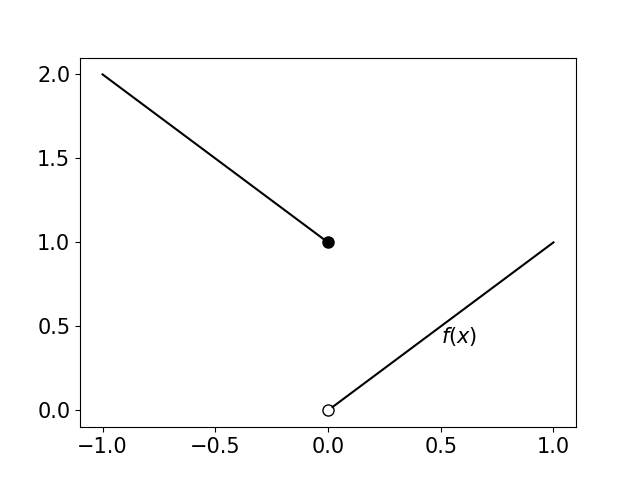
\includegraphics[width=0.4\textwidth]{figures/discontinuous_function.png}};
        \node at (7,0)
        {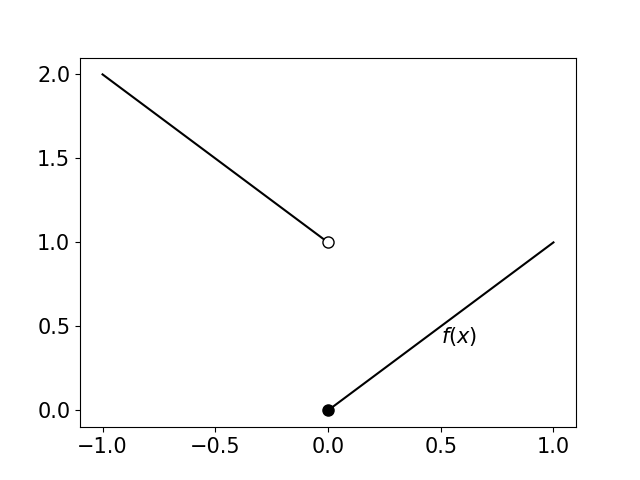
\includegraphics[width=0.4\textwidth]{figures/lsc_function.png}};
        \node at (0,-3) {Minimum tidak tercapai};
        \node at (7,-3) {Minimum tercapai};
    \end{tikzpicture}
    \caption{Kegagalan semikontinuitas bawah dapat menyebabkan infimum tidak
    tercapai.}
    \label{prelim:fig:lsc}
\end{figure}

\noindent\textbf{Deskripsi gambar.} Kedua panel menampilkan fungsi sepotong-sepotong
yang mempunyai lompatan di $x=0$. Pada panel kiri, cabang kanan mendekati titik
kosong $(0,0)$ sementara nilai fungsi di $x=0$ adalah titik penuh $(0,1)$;
infimum $0$ tidak tercapai. Pada panel kanan, titik $(0,0)$ diisi dan titik
$(0,1)$ dibiarkan kosong, sehingga nilai minimum $0$ tercapai.

% H01-S008 | sumber authority/habring/source-v1/preliminaries.tex baris 496--530
% segment-id: d90.hab.v1.ch01.seg0008
\begin{defn}[Koersif]
    Fungsi $f:V\rightarrow(-\infty,+\infty]$ disebut koersif jika
    \begin{equation}
        \lim_{\|x\|\rightarrow\infty}f(x)=\infty.
    \end{equation}
\end{defn}

\begin{theorem}\label{preliminaries:thm:direct_method}
    Misalkan $V$ berdimensi hingga dan
    $f:V\rightarrow(-\infty,\infty]$ proper, koersif, serta semikontinu bawah.
    Maka $f$ mencapai minimumnya pada $V$.\footnote{Asumsi dimensi hingga
    menyediakan kekompakan sekuensial yang dipakai bukti ini. Generalisasi ke
    dimensi tak hingga memerlukan hipotesis tambahan, misalnya refleksivitas dan
    semikontinuitas bawah lemah; ketiga asumsi yang ditampilkan saja tidak cukup.}
\end{theorem}

\begin{proof}
    Bukti mengikuti apa yang disebut \emph{metode langsung}.

    \paragraph{Langkah 1: Ambil barisan peminimum.}
    Misalkan $(x_n)_n$ suatu barisan peminimum\footnote{Sebagai latihan:
    mengapa barisan seperti ini selalu ada?}, yaitu
    \begin{equation}
        \lim_n f(x_n)=\inf_{x\in V}f(x).
    \end{equation}

    \paragraph{Langkah 2: Tunjukkan keterbatasan barisan.}
    Karena $f$ koersif, barisan peminimum harus terbatas. Jika tidak, terdapat
    subbarisan $(x_{n(k)})_k$ dengan $\|x_{n(k)}\|\rightarrow\infty$.
    Koersivitas kemudian memberikan
    \begin{equation}
        f(x_{n(k)})\rightarrow\infty,
    \end{equation}
    yang bertentangan dengan
    \begin{equation}
        f(x_{n(k)})\rightarrow\inf f<\infty.
    \end{equation}

    \paragraph{Langkah 3: Gunakan kekompakan untuk mengambil subbarisan
    konvergen.}
    Berdasarkan~\cref{thm:bolzano}, setiap barisan terbatas dalam ruang vektor
    berdimensi hingga mempunyai subbarisan konvergen. Jadi kita dapat mengambil
    subbarisan $(x_{n(k)})_k$ dengan limit
    $\lim_kx_{n(k)}=\hat x$.

    \paragraph{Langkah 4: Simpulkan dengan semikontinuitas bawah.}
    Berdasarkan semikontinuitas bawah $f$,
    \begin{equation}
        f(\hat x)
        \leq\liminf_{k\rightarrow\infty}f(x_{n(k)})
        =\lim_n f(x_n)
        =\inf_x f(x)
        \leq f(\hat x).
    \end{equation}
    Jadi semua ketaksamaan merupakan kesamaan dan $\hat x$ adalah peminim.
\end{proof}

\chapter{Kekonveksan}

% H02-S001 | sumber authority/habring/source-v1/convexity.tex baris 1--40
% segment-id: d90.hab.v1.ch02.seg0001
Tujuan kita dalam kuliah ini adalah menyelesaikan masalah berbentuk
\begin{equation}
    \min_{x\in C} f(x),
\end{equation}
dengan $C\subset V$ suatu \emph{himpunan bagian konveks} dari ruang $V$ dan $f:C\rightarrow (-\infty,\infty]$ suatu \emph{fungsi konveks}. Oleh karena itu, pada bagian berikut kita menganalisis secara lebih terperinci arti tepat kekonveksan himpunan dan fungsi serta akibat yang dapat ditarik dari sifat-sifat tersebut.

\section{Himpunan konveks}
Suatu himpunan disebut konveks apabila, untuk setiap dua titik di dalamnya, seluruh ruas garis lurus yang menghubungkan kedua titik itu juga termuat di dalam himpunan tersebut. Secara lebih formal:
\begin{defn}
    Suatu himpunan $C\subset V$ disebut konveks jika dan hanya jika, untuk setiap $x,y\in C$ dan $\lambda\in (0,1)$, berlaku
    \begin{equation}
        \lambda x + (1-\lambda) y\in C.
    \end{equation}
\end{defn}

Perhatikan bahwa
\begin{equation}
    \lambda x + (1-\lambda) y = y + \lambda(x-y),
\end{equation}
yang memperlihatkan dengan lebih jelas bahwa $\lambda x + (1-\lambda)y$ menelusuri ruas garis yang menghubungkan $x$ dan $y$.

Lebih lanjut, dengan menggunakan \emph{kombinasi konveks} yang lebih umum, kita dapat dengan mudah menunjukkan hasil berikut.

\begin{lemma}
    Himpunan $C\subset V$ konveks jika dan hanya jika, untuk setiap $n\in \N$, $x_i\in C$, dan $\lambda_i\in [0,1]$, $i=1,\dots,n$, yang memenuhi $\sum_{i=1}^n\lambda_i=1$, berlaku
    \begin{equation}
        \sum_{i=1}^n\lambda_i x_i \in C.
    \end{equation}
\end{lemma}
\begin{proof}
    Latihan.
\end{proof}

Untuk memudahkan notasi, kita mendefinisikan \emph{simpleks satuan} sebagai
\begin{equation}
    % Koreksi H02-C001 (sumber baris 37): batas penjumlahan n diganti k agar sesuai dengan Delta^k dan k komponen lambda.
    \Delta^k = \{(\lambda_1,\dots,\lambda_k)\in [0,1]^k\;|\;\sum_{i=1}^k\lambda_i = 1\}.
\end{equation}
Sekarang kita dapat mendefinisikan himpunan konveks terkecil yang memuat suatu himpunan, yaitu \emph{selubung konveks}.

% H02-S002 | sumber authority/habring/source-v1/convexity.tex baris 42--65
% segment-id: d90.hab.v1.ch02.seg0002
\begin{defn}[Selubung konveks]
    Misalkan $C\subset V$. Selubung konveks dari $C$ didefinisikan sebagai himpunan
    \begin{equation}\label{eq:convex_sets:defin_conv_hull}
        \conv(C) \coloneqq \bigcap_{\substack{S\subset V \text{ konveks}\\C\subset S}}S.
    \end{equation}
\end{defn}

\begin{lemma}
    Berlaku
    \begin{equation}\label{eq:convex_sets:conv_hull}
        % Koreksi H02-C028: vektor bobot ditulis lengkap, bukan skalar lambda.
        \conv(C) = \bigg\{ \sum_{i=1}^n\lambda_i x_i\;|\; n\in \N,\;x_i\in C, \;
        (\lambda_1,\ldots,\lambda_n)\in \Delta^n\bigg\}.
    \end{equation}
\end{lemma}
\begin{proof}
    Nyatakan ruas kanan \eqref{eq:convex_sets:conv_hull} dengan $A$.
    Kita akan menunjukkan bahwa $\conv(C)\subset A$ dan $A\subset\conv(C)$.

    \underline{$A\subset\conv(C)$:}
    Misalkan $x=\sum_{i=1}^n\lambda_i x_i\in A$. Untuk setiap $S\subset V$ yang konveks dan memenuhi $C\subset S$, berlaku $x\in S$. Oleh karena itu, berdasarkan definisi pada \eqref{eq:convex_sets:defin_conv_hull}, diperoleh $x\in\conv(C)$.

    \underline{$\conv(C)\subset A$:}
    Dapat diperiksa langsung bahwa $A$ memang merupakan himpunan konveks. Selain itu, $C\subset A$. Dengan demikian, $A$ termasuk salah satu himpunan $S$ dalam \eqref{eq:convex_sets:defin_conv_hull}, sehingga $\conv(C)\subset A$.
\end{proof}

% H02-S003 | sumber authority/habring/source-v1/convexity.tex baris 67--97
% segment-id: d90.hab.v1.ch02.seg0003
\begin{figure}
    \centering
    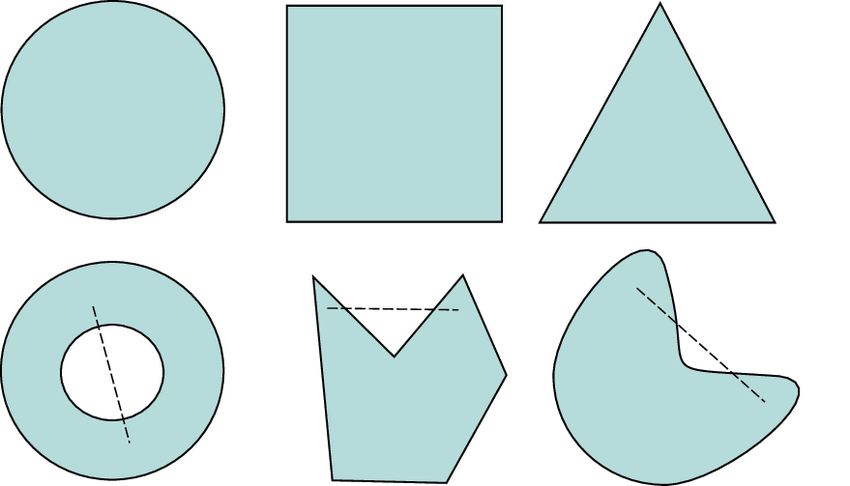
\includegraphics[width=.7\textwidth]{figures/sets.png}
    \caption{Baris atas: himpunan konveks. Baris bawah: himpunan tak konveks.}
\end{figure}

\noindent\textbf{Deskripsi gambar.} Baris atas memperlihatkan beberapa daerah yang memuat seluruh ruas garis di antara setiap dua titik di dalamnya. Baris bawah memperlihatkan daerah yang memiliki lekukan atau bagian terpisah sehingga terdapat dua titik di dalam himpunan yang ruas penghubungnya keluar dari himpunan.

\begin{example}
    Himpunan-himpunan berikut bersifat konveks (buktinya ditinggalkan sebagai latihan):
    \begin{itemize}
        \item Himpunan kosong $\emptyset$.
        \item Setiap ruang vektor.
        \item Setiap bola norma; yaitu, untuk setiap norma $\|\emptyarg\|$, setiap $c\in V$, dan setiap $R\geq 0$, himpunan
        \begin{equation}
            % Koreksi H02-C002 (sumber baris 80--82): tanda sama dengan yang hilang ditambahkan.
            B_{\|\emptyarg\|,R}(c)=\{x\in V\;|\; \|x-c\|<R\}
        \end{equation}
        dan
        \begin{equation}
            % Koreksi H02-C003 (sumber baris 84--86): tanda sama dengan yang hilang ditambahkan.
            \overline{B}_{\|\emptyarg\|,R}(c)=\{x\in V\;|\; \|x-c\|\leq R\}.
        \end{equation}
        \item Setiap subruang afin; yaitu, untuk setiap vektor $z,x_1,\dots,x_k\in V$, himpunan
        \begin{equation}
            \bigg\{ x\in V\;|\; x = z + \sum_{i=1}^k\lambda_i x_i,\; \lambda_i\in \R \bigg\}.
        \end{equation}
    \end{itemize}
\end{example}

\begin{figure}
    \centering
    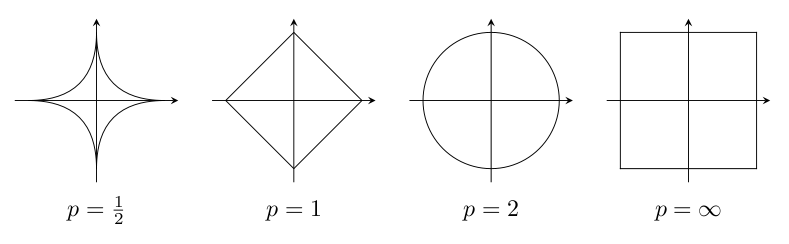
\includegraphics[width=1\textwidth]{figures/balls.png}
    \caption{Bola norma $\overline{B}_{\|\emptyarg\|_p,R}(0)$ untuk beberapa norma $\ell^p$. Perhatikan bahwa himpunan untuk $p=1/2$ tidak konveks karena pilihan ini tidak menghasilkan norma: ketaksamaan segitiga tidak berlaku.}
\end{figure}

\noindent\textbf{Deskripsi gambar.} Gambar membandingkan bola satuan dua dimensi untuk beberapa nilai $p$. Bentuknya berubah dari belah ketupat melalui lingkaran menuju bentuk yang semakin menyerupai persegi ketika $p$ bertambah; untuk $p=1/2$, sisi-sisinya melengkung ke dalam sehingga himpunannya tidak konveks.

% H02-S004 | sumber authority/habring/source-v1/convexity.tex baris 99--126
% segment-id: d90.hab.v1.ch02.seg0004
\begin{lemma}[Operasi yang mempertahankan kekonveksan]\label{convexity:lemma:ops preserving convexity}
    Pernyataan-pernyataan berikut berlaku:
    \begin{enumerate}
        \item Irisan. Misalkan $C_i\subset V$ konveks untuk $i\in I$, dengan $I$ suatu himpunan indeks sembarang. Maka irisan
        \begin{equation}
            \bigcap_{i\in I} C_i \coloneqq \{x\in V\;|\; x\in C_i\; \forall i\in I\}
        \end{equation}
        bersifat konveks.
        \item Jumlah berbobot. Misalkan $C_i\subset V$ konveks untuk $i=1,\dots,N$, dan misalkan $\lambda_i\in\R$ untuk $i=1,\dots,N$. Maka himpunan
        \begin{equation}
            % Koreksi H02-C004 (sumber baris 108--110): n dan indeks I yang tidak didefinisikan diseragamkan menjadi N dan i=1,...,N.
            \sum_{i=1}^N \lambda_i C_i \coloneqq \bigg\{\sum_{i=1}^N \lambda_i x_i\;|\; x_i\in C_i\; \forall i=1,\dots,N\bigg\}
        \end{equation}
        bersifat konveks.
        \item Produk Kartesius. Misalkan $C_i\subset V$ konveks untuk $i\in I$, dengan $I$ suatu himpunan indeks sembarang. Maka produk Kartesius
        \begin{equation}
            % Koreksi H02-C029: produk Kartesius memakai simbol produk, bukan produk tensor.
            \prod_{i\in I} C_i \coloneqq \{(x_i)_{i\in I}\;|\; x_i\in C_i\; \forall i\in I\}
        \end{equation}
        bersifat konveks.
        \item Citra dan pracitra\footnote{Pracitra terdefinisi dengan baik juga untuk pemetaan yang tidak invertibel.} di bawah pemetaan linear bersifat konveks. Secara khusus, untuk $A:V\rightarrow W$ linear serta $S\subset V$ dan $T\subset W$ keduanya konveks, himpunan-himpunan berikut bersifat konveks:
        \begin{equation}
            % Koreksi H02-C005 (sumber baris 120--122): pracitra diberi argumen T dan variabel himpunannya diperbaiki dari y menjadi x.
            A(S)=\{Ax\;|\;x\in S\},\qquad A^{-1}(T)=\{x\in V\;|\;Ax\in T\}.
        \end{equation}
    \end{enumerate}
\end{lemma}
\begin{proof}
    Kita hanya membuktikan bagian pertama dan meninggalkan sisanya sebagai latihan. Buktinya langsung. Misalkan $x,y\in\bigcap_{i\in I}C_i$ dan $\lambda\in(0,1)$. Karena $x,y\in C_i$ untuk setiap $i$ dan setiap $C_i$ konveks, diperoleh $\lambda x+(1-\lambda)y\in C_i$ untuk setiap $i$. Dengan demikian, $\lambda x+(1-\lambda)y\in\bigcap_{i\in I}C_i$.
\end{proof}

% H02-S005 | sumber authority/habring/source-v1/convexity.tex baris 128--191
% segment-id: d90.hab.v1.ch02.seg0005
Kita hendak mendefinisikan secara formal pengertian hiperbidang, yaitu perumuman bidang dua dimensi di $\R^3$ ke dimensi sembarang.

\begin{defn}[Hiperbidang]
    Misalkan $V$ suatu ruang hasil kali dalam. Hiperbidang adalah himpunan $H$ berbentuk
    \begin{equation}
        H=\{x\in V\;|\;\inner{x}{a}=b\}
    \end{equation}
    untuk suatu $a\in V\setminus\{0\}$ dan $b\in\R$.
\end{defn}

Parameter $a$ menentukan orientasi bidang dan $b$ menentukan geserannya. Secara khusus, $0\in H$ jika dan hanya jika $b=0$; dalam kasus ini $H$ merupakan subruang. Jika $b\neq0$, $H$ hanya merupakan subruang afin.

Perhatikan bahwa jika $x_0\in H$, maka
\begin{equation}
    H=\{x\in V\;|\;\inner{x-x_0}{a}=0\}.
\end{equation}
Jadi, $a$ adalah vektor normal terhadap bidang tersebut. Selain itu, dapat diperiksa sebagai latihan bahwa $\frac{|b|}{\|a\|}$ adalah jarak bidang dari titik asal.

Setiap hiperbidang membagi ruang menjadi dua setengah ruang.
\begin{defn}[Setengah ruang]
    Misalkan $V$ suatu ruang hasil kali dalam. Setengah ruang adalah himpunan $H^-$ berbentuk
    \begin{equation}
        H^-=\{x\in V\;|\;\inner{x}{a}\leq b\}
    \end{equation}
    untuk suatu $a\in V\setminus\{0\}$ dan $b\in\R$.
\end{defn}

Teorema berikut menyatakan bahwa pemisahan tersebut dapat dipilih dengan cara tertentu. Hasil ini ternyata sangat penting dalam optimisasi dan analisis fungsional.

\begin{theorem}[Teorema pemisahan Hahn--Banach]
    % Koreksi H02-C006 (sumber baris 156--166): ruang topologis, fungsional kontinu, dan ambang alpha yang semula dideklarasikan tetapi tidak dipakai dibuat eksplisit.
    Misalkan $S,T$ dua himpunan bagian konveks yang tak kosong dan saling lepas dari suatu ruang bernorma real $V$, dan misalkan $S$ terbuka. Maka terdapat $a\in V^*$ yang kontinu dan tak nol serta $\alpha\in\R$ sedemikian sehingga
    \begin{equation}
        \langle a,x\rangle<\alpha\leq\langle a,y\rangle,\qquad x\in S,\;y\in T.
    \end{equation}
    Jika $S$ dan $T$ keduanya tertutup dan salah satunya kompak, maka terdapat $a\in V^*$ yang kontinu dan tak nol, $\alpha\in\R$, dan $\epsilon>0$ sedemikian sehingga
    \begin{equation}
        \langle a,x\rangle\leq\alpha<\alpha+\epsilon\leq\langle a,y\rangle,\qquad x\in S,\;y\in T.
    \end{equation}
\end{theorem}
Versi kedua memungkinkan kita memperoleh selisih positif tegas antara
\[
    \sup_{x\in S}\langle a,x\rangle
    \quad
    \text{dan}
    \quad
    \inf_{y\in T}\langle a,y\rangle.
\]

\begin{figure}
    \centering
            \begin{tikzpicture}[font=\sffamily]
                \draw[dashed] (-2.5,3) -- (2.5,-0.5);
                \node[circle,draw,fill=gray,minimum size=2.4cm] at (1,2.4) {$S$};
                \draw[fill=gray,rounded corners] (-2,2) -- (-0.2,1) -- (0.2,-1) -- (-1.5,0) -- (-2.2,1.5) --cycle;
                \path (-2,2) --  (0.2,-1)  node[midway] {$T$};
                \draw[ultra thin] (-3,0) -- (3,0) (0,-2) -- (0,4);
            \end{tikzpicture}\hfill%
            \begin{tikzpicture}[font=\sffamily]
                \node[circle,draw,fill=gray,minimum size=2.4cm] at (1,2.4) {$S$};
                \draw[fill=gray,rounded corners] (0,4) -- (-0.5,1) -- (.5,.8) -- (2,.5) -- (0,-.5) -- (-1.5,0) -- (-2.2,1.5) --cycle;
                \path (-2,2) --  (0.2,-1)  node[midway] {$T$};
                \draw[ultra thin] (-3,0) -- (3,0) (0,-2) -- (0,4);
            \end{tikzpicture}
    \caption{Ilustrasi teorema pemisahan Hahn--Banach dan alasan pemisahan dapat gagal tanpa kekonveksan.}
\end{figure}

\noindent\textbf{Deskripsi gambar.} Panel kiri menampilkan dua himpunan konveks tak beririsan yang dipisahkan oleh sebuah garis putus-putus. Panel kanan menampilkan salah satu himpunan yang tak konveks dan melingkupi sebagian himpunan lainnya, sehingga tidak ada satu garis lurus yang dapat memisahkan keduanya.

\section{Fungsi konveks}

% H02-S006 | sumber authority/habring/source-v1/convexity.tex baris 193--261
% segment-id: d90.hab.v1.ch02.seg0006
Seperti diperlihatkan pada \cref{fig:convexity:1d_example}, kekonveksan sangat memengaruhi pertanyaan tentang keberadaan dan ketunggalan minimum.
\begin{figure}
    \centering
    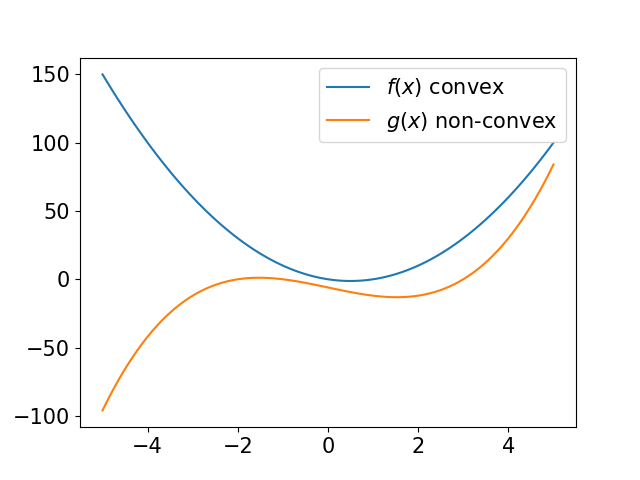
\includegraphics[width=0.5\textwidth]{figures/convex_fct.png}
    \caption{Contoh fungsi konveks dan fungsi tak konveks dalam satu dimensi.}
    \label{fig:convexity:1d_example}
\end{figure}

\noindent\textbf{Deskripsi gambar.} Gambar membandingkan grafik satu dimensi berbentuk mangkuk, yang konveks dan memiliki struktur minimum yang teratur, dengan grafik tak konveks yang memiliki lekukan serta beberapa minimum lokal.

\begin{defn}[Syarat orde nol untuk kekonveksan]
    Misalkan $C\subset V$ konveks dan $f:C\rightarrow(-\infty,\infty]$.
    \begin{itemize}
        \item Fungsi $f$ disebut konveks jika dan hanya jika, untuk setiap $x,y\in C$ dan $\lambda\in(0,1)$, berlaku
        \begin{equation}
            f(\lambda x+(1-\lambda)y)\leq\lambda f(x)+(1-\lambda)f(y).
        \end{equation}
        \item Fungsi $f$ disebut konveks tegas jika dan hanya jika, untuk setiap
        $x,y\in\dom(f)$ dengan $x\neq y$ dan setiap $\lambda\in(0,1)$, berlaku
        \begin{equation}
            % Koreksi H02-C007 (sumber baris 210--213): syarat x tidak sama dengan y ditambahkan; tanpa syarat ini ketaksamaan tegas mustahil saat x=y.
            f(\lambda x+(1-\lambda)y)<\lambda f(x)+(1-\lambda)f(y).
        \end{equation}
        \item Fungsi $f$ disebut konveks kuat dengan parameter $\mu>0$ jika dan
        hanya jika, untuk setiap $x,y\in\dom(f)$ dan $\lambda\in(0,1)$, berlaku
        % Koreksi H02-C025 (sumber baris 214): syarat mu>0 dibuat eksplisit; mu=0 hanya menghasilkan kekonveksan biasa.
        % Koreksi H02-C037: untuk fungsi nilai-diperluas, syarat tegas/kuat dibatasi pada domain efektif.
        \begin{equation}
            f(\lambda x+(1-\lambda)y)\leq\lambda f(x)+(1-\lambda)f(y)-\frac{\lambda(1-\lambda)\mu}{2}\|x-y\|^2.
        \end{equation}
    \end{itemize}
\end{defn}
Syarat orde nol menyatakan bahwa ruas garis yang menghubungkan dua titik pada grafik, yaitu garis sekan, selalu berada di atas fungsi. Untuk fungsi konveks tegas, garis sekan berada secara tegas di atas fungsi, sedangkan dalam kasus konveks kuat kita bahkan dapat \emph{menyisipkan} fungsi kuadrat di antara keduanya.

\begin{figure}
    \centering
    \begin{tikzpicture}[inner sep=.5mm,
            declare function={
                f(\x)= (\x-3)^2+3*\x-4;
            }
            ]
            \begin{axis}[axis lines=middle,domain=-1:4,samples=200,xtick={0.5,3},xticklabels={$x$,$y$},ytick=\empty,xmin=-.2,xmax=3.7,ymin=-.1,ymax=10]
                \addplot[blue,very thick,name path=f] {f(x)};
                \pgfplotsinvokeforeach{.5,3}{
                    \path[name path=x] (#1,0) -- (#1,6);
                    \draw[black!50,thick,dashed,name intersections={of=f and x, name=i}] (#1,0) -- (i-1);
                }
                \draw[very thick] ($(.5,{f(.5)})$) node[circle,fill=blue,label=left:{$f(x)$}]{} -- ($(3,{f(3)})$) node[circle,fill=blue,label=right:{$f(y)$}]{};
                \node[text=blue] at (1.75,2) {$f(\lambda x+(1-\lambda)y)$};
                \node[rotate=10] at (1.75,5) {$\lambda f(x)+(1-\lambda)f(y)$};
            \end{axis}
        \end{tikzpicture}
        \caption{Penafsiran geometris syarat orde nol bagi kekonveksan suatu fungsi.}
\end{figure}

\noindent\textbf{Deskripsi gambar.} Sebuah kurva konveks biru ditampilkan bersama dua titik pada grafik dan ruas sekan yang menghubungkannya. Nilai fungsi pada kombinasi konveks kedua titik berada di bawah nilai yang diperoleh melalui interpolasi linear di sepanjang sekan.

\begin{example}
    Fungsi-fungsi berikut konveks (bukti: latihan):
    \begin{enumerate}
        \item Fungsi afin $f(x)=\langle a,x\rangle+b$ dengan $a\in V^*$ dan $b\in\R$; khususnya, fungsi linear ketika $b=0$.
        % Koreksi H02-C008 (sumber baris 247): simbol y/a yang tidak konsisten diseragamkan menjadi a, dan koefisien dinyatakan sebagai fungsional linear a di V^*.
        \item Semua norma merupakan fungsi konveks.
    \end{enumerate}
\end{example}

Serupa dengan hasil untuk himpunan konveks, kekonveksan dapat diperluas ke kombinasi konveks dengan banyak titik yang sembarang.

\begin{theorem}[Jensen]
    % Koreksi H02-C026 (sumber baris 255): kodomain nilai-diperluas dibuat konsisten dan kasus bobot nol dinyatakan.
    Misalkan $C\subset V$ konveks dan
    $f:C\rightarrow(-\infty,+\infty]$. Dengan konvensi
    $0\cdot(+\infty)=0$, fungsi $f$ konveks jika dan hanya jika, untuk setiap
    $k\in\N$, $\lambda\in\Delta^k$, dan $x_i\in C$, berlaku
    \begin{equation}
        f\bigg(\sum_{i=1}^k\lambda_i x_i\bigg)\leq\sum_{i=1}^k\lambda_i f(x_i).
    \end{equation}
\end{theorem}

% H02-S007 | sumber authority/habring/source-v1/convexity.tex baris 262--322
% segment-id: d90.hab.v1.ch02.seg0007
Di atas kita melihat bahwa kekonveksan berarti garis sekan berada di atas fungsi. Kekonveksan juga berarti garis singgung berada di bawah fungsi (\cf~\cref{convexity:fig:gradients}).

\begin{theorem}[Karakterisasi orde pertama kekonveksan]\label{convexity:thm:first_order}
    % Koreksi H02-C030: turunan pada titik batas didefinisikan melalui perluasan ke lingkungan terbuka.
    Misalkan $C\subset\R^d$ konveks dan $f:C\rightarrow\R$ mempunyai perluasan
    yang terdiferensialkan secara kontinu pada suatu lingkungan terbuka dari $C$.
    \begin{itemize}
        \item Fungsi $f$ konveks jika dan hanya jika, untuk semua $x,y\in C$,
        \[
            f(x)+\langle\nabla f(x),y-x\rangle\leq f(y).
        \]
        \item Fungsi $f$ konveks tegas jika dan hanya jika ketaksamaan di atas berlaku tegas untuk semua $x\neq y$.
    \end{itemize}
\end{theorem}
\begin{proof}
    Kita terlebih dahulu membuktikan butir pertama.

    $\Rightarrow$: Misalkan $f$ konveks. Maka
    \begin{equation}
        f(x+\lambda(y-x))=f(\lambda y+(1-\lambda)x)\leq\lambda f(y)+(1-\lambda)f(x).
    \end{equation}
    Dengan menyusun ulang, diperoleh
    \begin{equation}
        \frac{f(x+\lambda(y-x))-f(x)}{\lambda}\leq f(y)-f(x).
    \end{equation}
    Membiarkan $\lambda\rightarrow0$ memberikan hasil yang diinginkan.

    $\Leftarrow$: Sekarang andaikan syarat gradien berlaku. Tuliskan $x_\lambda=x+\lambda(y-x)$. Maka
    \begin{equation*}
        f(x_\lambda)+\langle\nabla f(x_\lambda),y-x_\lambda\rangle
        =f(x_\lambda)+\langle\nabla f(x_\lambda),(1-\lambda)(y-x)\rangle\leq f(y)
    \end{equation*}
    dan
    \begin{equation*}
        f(x_\lambda)+\langle\nabla f(x_\lambda),x-x_\lambda\rangle
        =f(x_\lambda)+\langle\nabla f(x_\lambda),-\lambda(y-x)\rangle\leq f(x).
    \end{equation*}
    Kalikan ketaksamaan pertama dengan $\lambda$, ketaksamaan kedua dengan $1-\lambda$, lalu jumlahkan. Hasilnya
    \begin{equation*}
        f(x_\lambda)\leq\lambda f(y)+(1-\lambda)f(x).
    \end{equation*}

    % Koreksi H02-C036 (sumber baris 270 dan 273--274): bukti karakterisasi tegas yang hilang dilengkapi.
    Untuk butir kedua, arah dari syarat orde pertama tegas menuju kekonveksan
    tegas langsung mengikuti argumen yang sama. Sebaliknya, jika $f$ konveks
    tegas dan $x\neq y$, fungsi satu variabel
    $g(t)=f(x+t(y-x))$ konveks tegas pada $[0,1]$. Kemiringan sekan
    $(g(t)-g(0))/t$ tak menurun dalam $t>0$ dan, untuk setiap $t_0\in(0,1)$,
    bernilai tegas lebih kecil daripada $g(1)-g(0)$. Mengambil limit
    $t\downarrow0$ memberikan
    $\langle\nabla f(x),y-x\rangle< f(y)-f(x)$.
\end{proof}

\begin{figure}
    \centering
    \begin{tikzpicture}[inner sep=.5mm,
            declare function={
                f(\x)=  (\x-3)^2+3*\x-4;
            }
            ]
            \begin{axis}[axis lines=middle,domain=-1:4,samples=200,xtick={2},xticklabels={$x$},ytick=\empty,xmin=-.2,xmax=3.7,ymin=-.1,ymax=10]
                \addplot[blue,very thick,name path=f] {f(x)};
                \pgfplotsinvokeforeach{2}{
                    \path[name path=x] (#1,0) -- (#1,6);
                    \draw[black!50,thick,dashed,name intersections={of=f and x, name=i}] (#1,0) -- (i-1);
                }
                \addplot[very thick] {f(2)+1*(x-2)};
                \node[circle,fill=blue,label=above:{$f(x)$}] at ($(2,{f(2)})$) {};
                \node[text=blue,yshift=5mm] at ($(.5,{f(.5)})$) {$f$};
            \end{axis}
            \node[rotate=17,yshift=-3mm] at (6, 2.5) {$\textcolor{black}{y \mapsto f(x)+\inner{\nabla f(x)}{y-x}}$};
        \end{tikzpicture}
        \caption{Penafsiran geometris syarat orde pertama bagi fungsi konveks.}
        \label{convexity:fig:gradients}
\end{figure}

\noindent\textbf{Deskripsi gambar.} Grafik sebuah fungsi konveks ditampilkan bersama garis singgungnya pada titik $x$. Garis afin $y\mapsto f(x)+\langle\nabla f(x),y-x\rangle$ berada di bawah grafik fungsi di seluruh domain yang diperlihatkan.

% H02-S008 | sumber authority/habring/source-v1/convexity.tex baris 324--376
% segment-id: d90.hab.v1.ch02.seg0008
\begin{defn}[Minimum]
    % Koreksi H02-C021 (sumber baris 324--325): x^* dinyatakan berada di domain C.
    Misalkan $f:C\rightarrow\R$ dan $x^*\in C$.
    \begin{itemize}
        \item Titik $x^*$ disebut minimum lokal jika dan hanya jika terdapat $\epsilon>0$ sedemikian sehingga
        \[
            % Koreksi H02-C009 (sumber baris 328--330): pembanding dibatasi pada domain C.
            f(x^*)\leq f(x),\qquad \forall x\in B_\epsilon(x^*)\cap C.
        \]
        \item Titik $x^*$ disebut minimum global jika dan hanya jika
        \[
            f(x^*)\leq f(x),\qquad \forall x\in C.
        \]
    \end{itemize}
    Minimum disebut \emph{tegas} apabila ketaksamaan yang bersesuaian berlaku tegas untuk semua titik pembanding $x\neq x^*$.
    % Koreksi H02-C010 (sumber baris 336): pengecualian x=x^* dibuat eksplisit karena ketaksamaan tegas tidak mungkin berlaku di titik yang sama.
\end{defn}

Sekarang kita dapat membuktikan hasil penting pertama dalam optimisasi konveks.
\begin{prop}\label{convexity:prop:OC1}
    % Koreksi H02-C011 (sumber baris 340--342): asumsi bahwa f konveks ditambahkan; tanpa asumsi ini titik stasioner tidak harus menjadi minimum global.
    % Koreksi H02-C031: titik stasioner dinyatakan berada di domain dan hipotesis diferensial diselaraskan dengan teorema sebelumnya.
    Misalkan $C\subset\R^d$ konveks, $f:C\rightarrow\R$ konveks dan mempunyai
    perluasan yang terdiferensialkan secara kontinu pada suatu lingkungan
    terbuka dari $C$, serta $x^*\in C$. Jika $\nabla f(x^*)=0$, maka $x^*$
    adalah peminimum \textbf{global}.
\end{prop}
\begin{proof}
    Berdasarkan karakterisasi orde pertama kekonveksan,
    \begin{equation}
        f(x)\geq f(x^*)+\langle\nabla f(x^*),x-x^*\rangle
        =f(x^*)+0.
    \end{equation}
\end{proof}

Perhatikan bahwa kebalikan \cref{convexity:prop:OC1}, yaitu implikasi
\begin{equation}
    \text{$x^*$ adalah minimum}\Rightarrow\nabla f(x^*)=0,
\end{equation}
secara umum hanya benar apabila $x^*$ berada di interior $C$, yang dinyatakan dengan $C^\circ$; yaitu, terdapat $\epsilon>0$ sedemikian sehingga $B_\epsilon(x^*)\subset C$.

\begin{theorem}
    % Koreksi H02-C012 (sumber baris 357--359): domain Euklides dan asumsi kekonveksan f dibuat eksplisit agar ekuivalensi sah.
    Misalkan $C\subset\R^d$ konveks, $f:C\rightarrow\R$ konveks dan mempunyai
    perluasan yang terdiferensialkan secara kontinu pada suatu lingkungan
    terbuka dari $C$, serta $x^*\in C^\circ$. Maka $\nabla f(x^*)=0$ jika dan
    hanya jika $x^*$ adalah peminimum global.
\end{theorem}
\begin{proof}
    Satu arah mengikuti \cref{convexity:prop:OC1}. Untuk arah lainnya, andaikan $x^*$ suatu minimum. Untuk setiap $v\in\R^d$, jika $t>0$ cukup kecil, optimalitas memberikan
    \begin{equation}
        f(x^*+tv)-f(x^*)\geq0.
    \end{equation}
    Karena $t>0$, pembagian dengan $t$ menghasilkan
    \begin{equation}
        \frac{f(x^*+tv)-f(x^*)}{t}\geq0.
    \end{equation}
    Dengan membiarkan $t\rightarrow0$, diperoleh
    \begin{equation}
        \langle\nabla f(x^*),v\rangle\geq0.
    \end{equation}
    Karena $v$ sembarang, argumen yang sama dapat diterapkan pada $-v$. Hasilnya
    \[
        \langle\nabla f(x^*),v\rangle\leq0.
    \]

    Jadi $\langle\nabla f(x^*),v\rangle=0$ untuk setiap $v$, dan karenanya
    $\nabla f(x^*)=0$ (mengapa?).
\end{proof}

% H02-S009 | sumber authority/habring/source-v1/convexity.tex baris 378--403
% segment-id: d90.hab.v1.ch02.seg0009
Dalam satu dimensi, jika suatu fungsi terdiferensialkan, kekonveksannya dapat dikarakterisasi melalui kemonotonan turunannya. Dalam dimensi sembarang berlaku hasil berikut.

\begin{theorem}[Kemonotonan gradien]
    % Koreksi H02-C032: domain, perluasan diferensial, dan kuantifier x,y dibuat eksplisit.
    Misalkan $C\subset\R^d$ konveks dan $f:C\rightarrow\R$ mempunyai perluasan
    yang terdiferensialkan secara kontinu pada suatu lingkungan terbuka dari
    $C$. Maka $f$ konveks jika dan hanya jika, untuk setiap $x,y\in C$,
    \begin{equation}
        \langle\nabla f(x)-\nabla f(y),x-y\rangle\geq0.
    \end{equation}
\end{theorem}
\begin{proof}
    $\Rightarrow$: Andaikan $f$ konveks. Berdasarkan karakterisasi orde pertama kekonveksan,
    \begin{equation}
        \begin{aligned}
            &f(x)+\langle\nabla f(x),y-x\rangle\leq f(y),\\
            &f(y)+\langle\nabla f(y),x-y\rangle\leq f(x).
        \end{aligned}
    \end{equation}
    Menjumlahkan kedua ketaksamaan memberikan hasil yang diinginkan.

    $\Leftarrow$: Andaikan $\nabla f$ monoton. Berdasarkan teorema dasar kalkulus,
    \begin{equation}
        \begin{aligned}
            f(y)-f(x)
            &=\int_0^1\frac{\dd}{\dd t}f(x+t(y-x))\dd t\\
            &=\int_0^1\langle\nabla f(x+t(y-x)),y-x\rangle\dd t\\
            &=\int_0^1\langle\nabla f(x+t(y-x))-\nabla f(x),y-x\rangle\dd t+\langle\nabla f(x),y-x\rangle\\
            &=\int_0^1\frac{1}{t}\underbrace{\langle\nabla f(x+t(y-x))-\nabla f(x),t(y-x)\rangle}_{\geq0}\dd t+\langle\nabla f(x),y-x\rangle\\
            &\geq\langle\nabla f(x),y-x\rangle.
        \end{aligned}
    \end{equation}
    Pada $t=0$, integran dipahami melalui perpanjangan kontinu; ketaksamaan monoton digunakan untuk $t\in(0,1]$.
\end{proof}

% H02-S010 | sumber authority/habring/source-v1/convexity.tex baris 405--453
% segment-id: d90.hab.v1.ch02.seg0010
Terakhir, turunan kedua juga dapat digunakan untuk mengarakterisasi kekonveksan. Secara intuitif, kekonveksan berarti \emph{kelengkungan positif}. Untuk memformalkan hal ini, ingat kembali cara mengurutkan matriks. Untuk dua matriks simetris $A,B\in\R^{d\times d}$, kita menuliskan
    % Koreksi H02-C022 (sumber baris 407--414): A dan B dinyatakan simetris karena urutan Loewner digunakan pada matriks simetris.
\begin{equation}
    A\succeq B\Longleftrightarrow\langle x,Ax\rangle\geq\langle x,Bx\rangle,\quad\forall x\in\R^d
\end{equation}
dan, serupa dengan itu,
\begin{equation}
    % Koreksi H02-C013 (sumber baris 411--413): x=0 dikecualikan dari urutan positif tegas.
    A\succ B\Longleftrightarrow\langle x,Ax\rangle>\langle x,Bx\rangle,\quad\forall x\in\R^d\setminus\{0\}.
\end{equation}

\begin{theorem}[Karakterisasi orde kedua kekonveksan]
    % Koreksi H02-C027 (sumber baris 416--417): C dinyatakan terbuka di R^d; tanpa domain berdimensi penuh, Hessian pada arah normal tidak mengarakterisasi kekonveksan restriksi.
    Misalkan $C\subset\R^d$ terbuka dan konveks, serta $f:C\rightarrow\R$ terdiferensialkan secara kontinu dua kali.
    \begin{enumerate}
        \item Fungsi $f$ konveks jika dan hanya jika $\nabla^2f(x)\succeq0$ untuk setiap $x\in C$.
        \item Jika $\nabla^2f(x)\succ0$ untuk setiap $x\in C$, maka $f$ konveks tegas.
        % Koreksi H02-C014 (sumber baris 420): ekuivalensi yang salah diganti dengan implikasi; fungsi x^4 konveks tegas tetapi Hessian-nya nol di x=0.
    \end{enumerate}
\end{theorem}
\begin{proof}
    Kita membuktikan pernyataan pertama dan arah cukup pada pernyataan kedua.

    $\Rightarrow$: Andaikan $f$ konveks. Berdasarkan kemonotonan gradien, untuk $t>0$ berlaku
    \begin{equation}
        \frac{\inner{\nabla f(x+tv)-\nabla f(x)}{v}}{t}\geq0.
    \end{equation}
    Dengan membiarkan $t\rightarrow0$, diperoleh
    \begin{equation}
        \langle v,\nabla^2f(x)v\rangle\geq0.
    \end{equation}
    Karena $v$ sembarang, hasilnya mengikuti.

    $\Leftarrow$: Andaikan $\nabla^2f\succeq0$. Berdasarkan teorema dasar kalkulus,
    \begin{equation}
        \begin{aligned}
            \nabla f(y)-\nabla f(x)
            &=\int_0^1\frac{\dd}{\dd t}\nabla f(x+t(y-x))\dd t\\
            &=\int_0^1\nabla^2f(x+t(y-x))(y-x)\dd t.
        \end{aligned}
    \end{equation}
    Mengambil hasil kali dalam dengan $y-x$ menghasilkan
    \begin{equation}
        \begin{aligned}
            % Koreksi H02-C015 (sumber baris 444--449): integran vektor yang salah pada ruas kanan diganti dengan bentuk kuadratik skalar.
            \langle\nabla f(y)-\nabla f(x),y-x\rangle
            &=\int_0^1\underbrace{\langle y-x,\nabla^2f(x+t(y-x))(y-x)\rangle}_{\geq0}\dd t\\
            &\geq0.
        \end{aligned}
    \end{equation}
    Kemonotonan gradien kini menyiratkan kekonveksan. Untuk membuktikan bagian
    tegas, tuliskan $d=y-x\neq0$. Jika Hessian positif definit pada setiap titik,
    maka
    \[
        f(y)-f(x)-\langle\nabla f(x),d\rangle
        =\int_0^1\int_0^t
        \langle d,\nabla^2f(x+sd)d\rangle\,\dd s\,\dd t>0.
    \]
    Jadi ketaksamaan orde pertama berlaku tegas dan $f$ konveks tegas.
\end{proof}

% \subsubsection{Operasi yang mempertahankan kekonveksan}

% H02-S011 | sumber authority/habring/source-v1/convexity.tex baris 457--484
% segment-id: d90.hab.v1.ch02.seg0011
\begin{lemma}[Operasi yang mempertahankan kekonveksan]
    Misalkan $f,f_1,\dots,f_n:C\rightarrow\R$ konveks pada suatu himpunan konveks.
    \begin{enumerate}
        \item Untuk setiap $\alpha\geq0$, fungsi $\alpha f$ konveks.
        \item Fungsi $\sum_i f_i$ konveks.
    \end{enumerate}
\end{lemma}
\begin{proof}
    Latihan.
\end{proof}

\begin{lemma}[Operasi yang mempertahankan kekonveksan, lanjutan]
    Misalkan $f:\R^n\supset C\rightarrow\R$ konveks, $A\in\R^{n\times m}$, dan $b\in\R^n$. Maka
    \begin{equation}
        g(x)=f(Ax+b)
    \end{equation}
    konveks pada $\{x\in\R^m\;|\;Ax+b\in C\}$.
\end{lemma}
\begin{proof}
    Latihan.
\end{proof}

\begin{lemma}[Operasi yang mempertahankan kekonveksan, lanjutan]
    Misalkan $f:C\rightarrow\R$ konveks dan $g:I\rightarrow\R$ konveks serta tak menurun, dengan $I\subset\R$ suatu interval yang memenuhi $f(C)\subset I$. Maka $g\circ f$ konveks.
\end{lemma}
\begin{proof}
    Latihan.
\end{proof}

% H02-S012 | sumber authority/habring/source-v1/convexity.tex baris 486--543
% segment-id: d90.hab.v1.ch02.seg0012
\begin{example}
    \begin{enumerate}
        \item Fungsi \emph{log-sum-exp} bersifat konveks:
        \begin{equation}
            f(x)=\log\bigg(\sum_{i=1}^n e^{x_i}\bigg).
        \end{equation}
        \item Fungsi kuadratik-per-linear
        \begin{equation}
            f(x)=\frac{x_1^2}{x_2}
        \end{equation}
        konveks pada $\R\times(0,\infty)$.
        \item Fungsi $h(x)=e^{\|x\|^2}$ konveks pada $\R^d$ karena $f(x)=\|x\|^2$ konveks dan $g(t)=e^t$ konveks serta tak menurun.
        \item Pertimbangkan $h(x)=(\|x\|^2+1)^2$ pada $\R^d$. Fungsi $f(x)=\|x\|^2+1$ dan $g(t)=t^2$ keduanya konveks. Fungsi $g$ tidak tak menurun pada seluruh $\R$, tetapi tak menurun pada $f(\R^d)=[1,\infty)$. Akibatnya, $h$ konveks.
        \item Pada contoh sebelumnya, jika $f$ diganti dengan $\|\emptyarg\|^2-1$, maka $g$ tidak tak menurun pada $f(\R^d)=[-1,\infty)$; lihat \cref{convexity:fig:compositions}.
        % Koreksi H02-C033: dimensi domain fungsi diseragamkan dari n menjadi d.
    \end{enumerate}
\end{example}

\begin{figure}
    \centering
    \begin{tikzpicture}[declare function={
            f1(\x) =  \x^2 + 1;
            f2(\x) =  \x^2 - 1;
            g(\x) = \x^2;
            h1(\x) = g(f1(\x));
            h2(\x) = g(f2(\x));
        }
        ]
        \begin{groupplot}[
            group style={group size= 3 by 1,vertical sep=1.5cm}, height=4.5cm, width=5.3cm,ymin=-1.2,ymax=2.5,domain=-2:2,xmin=-1.6,xmax=1.6,samples=200,grid
        ]
            \nextgroupplot[
                align=center,
                title={%
                    \( \textcolor{teal}{f_1 : x \mapsto x^2 + 1} \) \\
                    \( \textcolor{red}{f_2 : x \mapsto x^2 - 1} \)
                }
            ]
                \addplot[teal, very thick] {f1(x)};
                \addplot[red, very thick] {f2(x)};
            \nextgroupplot[title={\( g : x \mapsto x^2\)}]
                \draw[->, teal, very thick] (axis cs:1, 0) -- (axis cs:1.5, 0) node [midway, above] {\( \textcolor{teal}{f_1(\R)} \)};
                \draw[->, red, very thick] (axis cs:-1, 0) -- (axis cs:.5, 0) node [midway, below] {\( \textcolor{red}{f_2(\R)} \)};
                \addplot[blue, very thick] {g(x)};
            \nextgroupplot[
                align=center,
                title={%
                    \( \textcolor{teal}{g \circ f_1 } \) \\
                    \( \textcolor{red}{g \circ f_2 } \)
                }
            ]
                \addplot[teal, very thick] {h1(x)};
                \addplot[red, very thick] {h2(x)};
        \end{groupplot}
    \end{tikzpicture}
    \caption{Kekonveksan komposisi fungsi.}
    \label{convexity:fig:compositions}
\end{figure}

\noindent\textbf{Deskripsi gambar.} Panel kiri menampilkan $f_1(x)=x^2+1$ dan $f_2(x)=x^2-1$. Panel tengah menampilkan $g(t)=t^2$ serta rentang kedua fungsi tersebut; $g$ tak menurun pada rentang $f_1$ tetapi tidak pada seluruh rentang $f_2$. Panel kanan memperlihatkan bahwa $g\circ f_1$ konveks, sedangkan $g\circ f_2$ memiliki lekukan tak konveks di sekitar titik asal.

% H02-S013 | sumber authority/habring/source-v1/convexity.tex baris 545--564
% segment-id: d90.hab.v1.ch02.seg0013
\begin{lemma}[Operasi yang mempertahankan kekonveksan, lanjutan]
    Misalkan $f_i:C\rightarrow\R$, $i=1,\dots,n$, konveks pada himpunan konveks $C$. Maka
    \begin{equation}
        f(x)=\max_{i=1,\dots,n}f_i(x)
    \end{equation}
    konveks.
\end{lemma}
\begin{proof}
    Kita hitung langsung:
    \begin{equation}
        \begin{aligned}
            f(\lambda x+(1-\lambda)y)
            &=\max_i f_i(\lambda x+(1-\lambda)y)\\
            &\leq\max_i\{\lambda f_i(x)+(1-\lambda)f_i(y)\}\\
            &\leq\lambda\max_jf_j(x)+(1-\lambda)\max_jf_j(y)\\
            &=\lambda f(x)+(1-\lambda)f(y).
        \end{aligned}
    \end{equation}
\end{proof}

% H02-S014 | sumber authority/habring/source-v1/convexity.tex baris 566--596
% segment-id: d90.hab.v1.ch02.seg0014
\begin{theorem}\label{convexity:thm:minimum}
    Misalkan $f:C\times D\rightarrow\R$ konveks pada $C\times D$, dengan $C$ dan $D$ keduanya konveks. Definisikan
    \begin{equation}
        g(x)=\inf_{y\in D}f(x,y),
    \end{equation}
    dan andaikan infimum tersebut hingga untuk setiap $x\in C$. Maka $g$ konveks.
\end{theorem}
\begin{proof}
    Pilih barisan $y_n^x$ dan $y_n^z$ sedemikian sehingga
    \begin{equation}
        g(x)=\lim_n f(x,y_n^x),\qquad g(z)=\lim_n f(z,y_n^z).
    \end{equation}
    Maka
    \begin{equation}
        \begin{aligned}
            g(\lambda x+(1-\lambda)z)
            &\leq f(\lambda x+(1-\lambda)z,\lambda y_n^x+(1-\lambda)y_n^z)\\
            &\leq\lambda f(x,y_n^x)+(1-\lambda)f(z,y_n^z).
        \end{aligned}
    \end{equation}
    Mengambil limit ketika $n\rightarrow\infty$ menyelesaikan bukti.
\end{proof}

\begin{example}
    % Koreksi H02-C016 (sumber baris 589--595): C harus tak kosong dan konveks; jarak ke himpunan tak konveks tidak selalu konveks.
    Jarak suatu titik ke himpunan tak kosong dan konveks merupakan fungsi konveks. Jadi, untuk setiap himpunan tak kosong dan konveks $C\subset\R^d$, pemetaan berikut konveks:
    \begin{equation}
        \begin{aligned}
            x\mapsto d(x,C)\coloneqq\inf_{y\in C}\|x-y\|.
        \end{aligned}
    \end{equation}
\end{example}

% H02-S015 | sumber authority/habring/source-v1/convexity.tex baris 598--624
% segment-id: d90.hab.v1.ch02.seg0015
\begin{theorem}
    % Koreksi H02-C017 (sumber baris 598--606): klausa g konveks dan domain garis yang berada di C ditambahkan; rumus sumber berakhir tanpa predikat dan memakai seluruh R walau x+tv dapat keluar dari C.
    Misalkan $C\subset\R^d$ konveks dan $f:C\rightarrow\R$. Maka $f$ konveks jika dan hanya jika, untuk setiap $x\in C$ dan $v\in\R^d$, fungsi
    \begin{equation}
        \begin{aligned}
            g:I_{x,v}&\rightarrow\R,\\
            t&\mapsto g(t)=f(x+tv),
        \end{aligned}
    \end{equation}
    konveks pada interval $I_{x,v}\coloneqq\{t\in\R\mid x+tv\in C\}$.
\end{theorem}
\begin{proof}
    $\Leftarrow$: Andaikan $g$ konveks untuk setiap $x$ dan $v$. Misalkan $x,y\in C$ dan $\lambda\in(0,1)$. Pertimbangkan
    \begin{equation}
        g(t)=f(y+t(x-y)).
    \end{equation}
    Karena $g$ konveks pada interval yang memuat $0$ dan $1$,
    \begin{equation}
        \begin{aligned}
            f(\lambda x+(1-\lambda)y)
            =g(\lambda)
            &=g(\lambda\cdot1+(1-\lambda)\cdot0)\\
            &\leq\lambda g(1)+(1-\lambda)g(0)\\
            &=\lambda f(x)+(1-\lambda)f(y).
        \end{aligned}
    \end{equation}
    Arah sebaliknya ditinggalkan sebagai latihan.
\end{proof}

% H02-S016 | sumber authority/habring/source-v1/convexity.tex baris 626--681
% segment-id: d90.hab.v1.ch02.seg0016
\begin{example}[Fungsi konveks yang umum]
    % Koreksi H02-C023 (sumber baris 626): garis miring terbalik yatim setelah pembuka lingkungan example dihapus.
    \begin{itemize}
        \item Contoh pada $\R$:
        \begin{itemize}
            \item Fungsi konveks:
            \begin{itemize}
                \item Fungsi eksponensial $f(x)=\exp(ax)$ pada $\R$, dengan $a\in\R$.
                \item Fungsi pangkat $f(x)=x^p$ pada $(0,\infty)$ untuk $p\geq1$ atau $p\leq0$.
                \item Pangkat nilai mutlak $f(x)=|x|^p$ pada $\R$ untuk $p\geq1$.
                \item Entropi negatif $f(x)=x\log(x)$ pada $(0,\infty)$.
            \end{itemize}
            \item Fungsi konkaf:
            \begin{itemize}
                \item Fungsi pangkat $f(x)=x^p$ pada $(0,\infty)$ untuk $0\leq p\leq1$.
                \item Logaritma $f(x)=\log(x)$ pada $(0,\infty)$.
            \end{itemize}
        \end{itemize}
        \item Contoh pada ruang Euklides berdimensi hingga:
        \begin{itemize}
            \item Fungsi konveks:
            \begin{itemize}
                \item Norma-$p$, $f(x)=\|x\|_p$.
                \item Pangkat norma-$p$, $f(x)=\|x\|_p^p$, untuk
                $1\leq p<\infty$.
                % Koreksi H02-C034: p=infinity dikecualikan karena pangkat tak hingga tidak terdefinisi.
                \item Kuadrat terkecil, $f(x)=\frac12\|Ax-b\|_2^2$, dengan $A\in\R^{m\times n}$ dan $b\in\R^m$.
                \item Maksimum fungsi-fungsi afin:
                    \[
                        f(x)=\max\{\inner{a_1}{x}+b_1,\ldots,\inner{a_m}{x}+b_m\},
                    \]
                dengan $a_i\in\R^n$ dan $b_i\in\R$.
                \item Perspektif suatu fungsi, $f(x,y)=yg(x/y)$, dengan
                $g:\R^n\rightarrow\R$ fungsi konveks, $x\in\R^n$, dan
                $y\in(0,\infty)$. Jadi domain perspektif ini adalah
                $\R^n\times(0,\infty)$.
                % Koreksi H02-C038: domain perspektif dibedakan dari domain R^n pada judul daftar sumber.
            \end{itemize}
            \item Fungsi konkaf:
            \begin{itemize}
                \item Minimum fungsi-fungsi afin:
                    \[
                        f(x)=\min\{\inner{a_1}{x}+b_1,\ldots,\inner{a_m}{x}+b_m\}.
                    \]
            \end{itemize}
        \end{itemize}
        \item Contoh pada $\R^{m\times n}$:
        \begin{itemize}
            \item Fungsi konveks:
            \begin{itemize}
                \item Fungsi afin
                    \[
                        f(X)=\tr(A^\top X)+b=\sum_{i=1}^m\sum_{j=1}^n A_{ij}X_{ij}+b
                    \]
                    pada $\R^{m\times n}$, dengan $A\in\R^{m\times n}$ dan $b\in\R$.
                    % Koreksi H02-C018 (sumber baris 669--673): dimensi A diperbaiki dari n x m menjadi m x n agar A^T X dan penjumlahan A_ij X_ij terdefinisi.
                \item Norma spektral $f(X)=\|X\|_2=\sigma_{\text{max}}(X)=\sqrt{\lambda_{\text{max}}(X^\top X)}$.
                \item Fungsi penghalang untuk matriks definit positif, $f(X)=-\log\det X$ pada $\mathbb{S}_{++}^n$.
            \end{itemize}
        \end{itemize}
    \end{itemize}
\end{example}

% H02-S017 | sumber authority/habring/source-v1/convexity.tex baris 683--699
% segment-id: d90.hab.v1.ch02.seg0017
Serupa dengan hasil-hasil di atas, kita dapat menunjukkan karakterisasi kekonveksan kuat berikut.

\begin{theorem}
    % Koreksi H02-C024 (sumber baris 683--697): domain Euklides dan syarat mu>0 dibuat eksplisit; setiap syarat diferensial diberi domain yang tepat.
    Misalkan $f:C\rightarrow\R$, dengan $C\subset\R^d$ konveks, serta
    $\mu>0$. Karakterisasi berikut berlaku:
    \begin{itemize}
        \item Fungsi $f$ konveks kuat berparameter $\mu$ jika dan hanya jika
        $f-\frac{\mu}{2}\|\emptyarg\|^2$ konveks.
        % Koreksi H02-C019 (sumber baris 686): faktor mu yang hilang dipulihkan.
        \item \emph{Syarat orde pertama}: jika $f$ mempunyai perluasan yang
        terdiferensialkan secara kontinu pada suatu lingkungan terbuka dari
        $C$, maka $f$ konveks kuat berparameter $\mu$ jika dan hanya jika, untuk
        setiap $x,y\in C$,
        \[
            f(x)+\inner{\nabla f(x)}{y-x}\leq f(y)-\frac{\mu}{2}\|x-y\|^2.
        \]
        \item \emph{Syarat orde kedua}: jika $C$ terbuka dan $f$
        terdiferensialkan secara kontinu dua kali pada $C$, maka $f$ konveks
        kuat berparameter $\mu$ jika dan hanya jika, untuk setiap $x\in C$,
        \[
            \nabla^2 f(x)\succeq\mu I.
        \]
        % Koreksi H02-C020 (sumber baris 691--694): skalar mu diganti mu I agar perbandingan matriks terdefinisi.
        % Koreksi H02-C035: setiap butir dinyatakan sebagai ekuivalensi dengan hipotesis regularitasnya sendiri.
    \end{itemize}
\end{theorem}
\begin{proof}
    Buktinya merupakan penyesuaian langsung dari bukti untuk kekonveksan biasa dan ditinggalkan sebagai latihan.
\end{proof}


\backmatter
\chapter*{Catatan koreksi terhadap sumber}
Terjemahan ini mempertahankan isi sumber kecuali pada koreksi yang dapat
ditentukan berikut. Koreksi dilakukan oleh penyusun edisi bahasa Indonesia dan
bukan perubahan yang disahkan oleh penulis sumber. Rekaman terstruktur lengkap
dengan pelacak sumber, alasan, dan disposisi menyertai edisi ini dalam
\texttt{00\_control/ADVERSE\_LEDGER.jsonl}.

\begin{enumerate}
    \item Tipe operasi ruang vektor, hukum distributif, kodomain norma, norma
    operator terinduksi, serta definisi ruang $L^p$ dan supremum esensial
    dibetulkan agar terdefinisi secara matematis.
    \item Kuantifier hasil kali dalam, bukti Cauchy--Schwarz, kasus ujung
    H\"older, ketaksamaan Young, dan kasus nol dalam bukti Minkowski dilengkapi.
    \item Bukti Bolzano--Weierstrass, definisi dual kontinu, representasi Riesz,
    eksistensi adjoin, dan hukum komposisi adjoin diperbaiki pada titik salah
    tipe atau hipotesis yang hilang.
    \item Semikontinuitas bawah, koersivitas, dan metode langsung diberi
    penanganan nilai tak hingga dan lingkup berdimensi hingga yang tepat.
    \item Simpleks, selubung konveks, bola norma, jumlah berbobot, produk
    Kartesius, pracitra, dan teorema pemisahan dibetulkan pada indeks, tanda,
    tipe, atau hipotesis yang dapat ditentukan.
    \item Kekonveksan tegas dan kuat dibatasi pada domain efektif bila fungsi
    bernilai diperluas; koefisien afin, konvensi Jensen, dan syarat titik
    pembanding minimum dibuat eksplisit.
    \item Karakterisasi orde pertama, kemonotonan gradien, dan syarat
    stasioneritas diberi domain Euklides serta hipotesis keterdiferensialan dan
    kekonveksan yang diperlukan.
    \item Urutan L\"owner, karakterisasi Hessian, operasi komposisi, dimensi
    matriks, jarak ke himpunan, dan restriksi pada garis diperbaiki agar semua
    pernyataan sah dan bertipe konsisten.
    \item Karakterisasi kekonveksan kuat memulihkan faktor $\mu$, matriks
    $\mu I$, rentang pangkat norma, dan struktur ekuivalensi sesuai regularitas.
\end{enumerate}

\chapter*{Atribusi, lisensi, dan nondukungan}
Karya sumber: Andreas Habring, \emph{Lecture Notes: Convex Optimization},
arXiv:2607.11664v1, 13 Juli 2026,
\url{https://arxiv.org/abs/2607.11664v1}. Karya sumber tersedia berdasarkan
Creative Commons Attribution 4.0 International (CC BY 4.0),
\url{https://creativecommons.org/licenses/by/4.0/}.

Edisi bahasa Indonesia ini merupakan karya turunan. Hak cipta materi sumber
tetap pada pemegang haknya. Anda boleh membagikan dan mengadaptasinya dengan
atribusi yang sesuai, tautan lisensi, dan penandaan perubahan sebagaimana
disyaratkan CC BY 4.0. Koreksi dan deskripsi akses baru dalam edisi ini juga
ditawarkan berdasarkan CC BY 4.0 sejauh hak terpisah dapat berlaku; bagian
sumber tetap CC BY 4.0.

Andreas Habring dan TU Graz tidak menyusun, memeriksa, menyetujui, atau
mendukung terjemahan ini. Penyebutan nama mereka semata-mata untuk atribusi
karya sumber.

\end{document}
